\chapter{Voruntersuchungen}
\label{chap:voruntersuchungen}
% Inhalt (Gliederung Kapitel 4, etwa 8 S.).

% Entwurf 4.1 (2026-10-17), Claude entwirft, der Nutzer redigiert.
% Schlüssel: Stommel, Stojek, Korte 2018 steht in der BA-Bib unter Sto18 (Sto18 ist dort
% Stoffregen, Motorradtechnik); hier wird Sto18 zitiert, damit der Eintrag auflöst.
\section{Netzkonvergenz und Elementtyp}
\label{sec:netzkonvergenz}

Vor dem Einfrieren des Radnetzes wurden Diskretisierung und Elementformulierung geprüft. Einer unzureichenden Diskretisierung begegnet nach Stommel, Stojek und Korte die h-Methode, bei der das Netz verfeinert wird, bis sich die Ergebnisse benachbarter Stufen nur noch wenig ändern \cite[S.~424]{Sto18}. Die Konvergenzstudie läuft vor der eigentlichen Auswertung an einem kleinen Modell unter vergleichbarer Last mit mehreren Elementtypen gegen eine Referenz \cite[S.~433]{Sto18}. Die Elementgröße wird dabei so groß gewählt, wie die Beanspruchungsgradienten es zulassen \cite[S.~465]{Sto18}. Als kleines Modell dient der Stirnschnitt des Radsektors im ebenen Dehnungszustand, weil das Volumennetz ein Auszug dieses Schnitts über die Zahnbreite ist. Gerechnet wird mit dem eigenen ebenen Löser aus \secref{sec:fe_modell}. Die Vollversion von Abaqus bestätigte jede Verfeinerungsstufe auf $0{,}01$\,MPa.

\figref{fig:lastfall_eben} zeigt den Lastfall. Die Last von $16$\,Nm am Rad wirkt am äußeren Einzeleingriffspunkt B mit dem längsten Hebelarm auf einen Zahn, als Linienlast von $43{,}66$\,N/mm. Sie ist als Hertzsche Pressungsverteilung nach \cite{Nie19} mit der halben Druckbreite $0{,}322$\,mm und der größten Pressung $86{,}4$\,MPa normal zur Flanke aufgebracht. Der Werkstoff ist isotrop mit dem Elastizitätsmodul $E = 2282$\,MPa bei $80$\,\textdegree C und der Querkontraktionszahl $0{,}30$, Bohrung und Schnittebenen sind fest. Bewertet werden die größte Hauptspannung $\sigma_{\mathrm{1}}$ an der Fußoberfläche der belasteten Flanke als Knotenmittel, die Verschiebung der Kopfmitte und die Formänderungsenergie des Sektors. Das Ausgangsnetz, das Netz des Referenzmodells der FVA-Workbench, hat 20 Elemente über der Zahnhöhe, 80 je Zahnlücke am Fuß und 10 über der Zahndicke. Verfeinert wurde gleichmäßig bis auf ein Viertel der Elementgröße und jede der drei Richtungen für sich. Der Grenzwert für die Elementgröße null folgt nach Richardson aus den letzten drei Stufen mit dem Ansatz
\begin{equation}
	f(h) = f_{\mathrm{0}} + C\,h^{p},
	\label{eq:richardson}
\end{equation}
wobei der Exponent $p$, die Konvergenzordnung der FE-Lösung \cite[S.~244]{Bat96}, aus den Stufen mitbestimmt wird \cite[S.~523]{DahReu22}.

\begin{figure}[htbp]
	\centering
	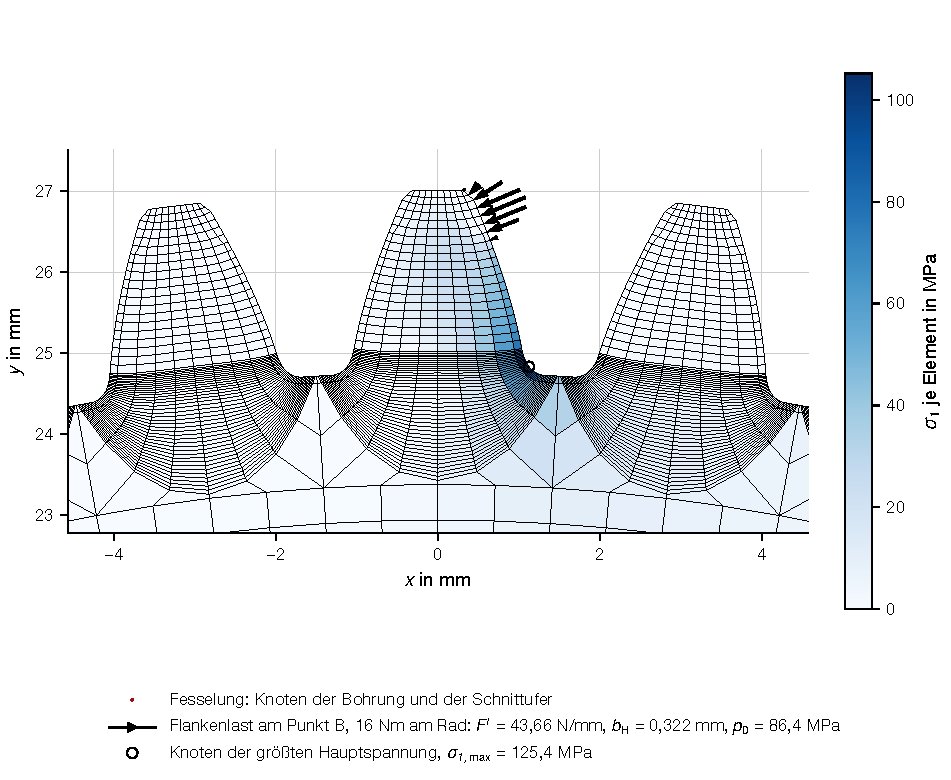
\includegraphics[width=0.8\textwidth]{kap4/lastfall_eben}
	\caption{Lastfall der Konvergenzstudie am ebenen Radsektor: Pressungsverteilung am Punkt B bei $16$\,Nm am Rad und größte Hauptspannung je Element im Ausgangsnetz.}
	\label{fig:lastfall_eben}
\end{figure}

\begin{figure}[htbp]
	\centering
	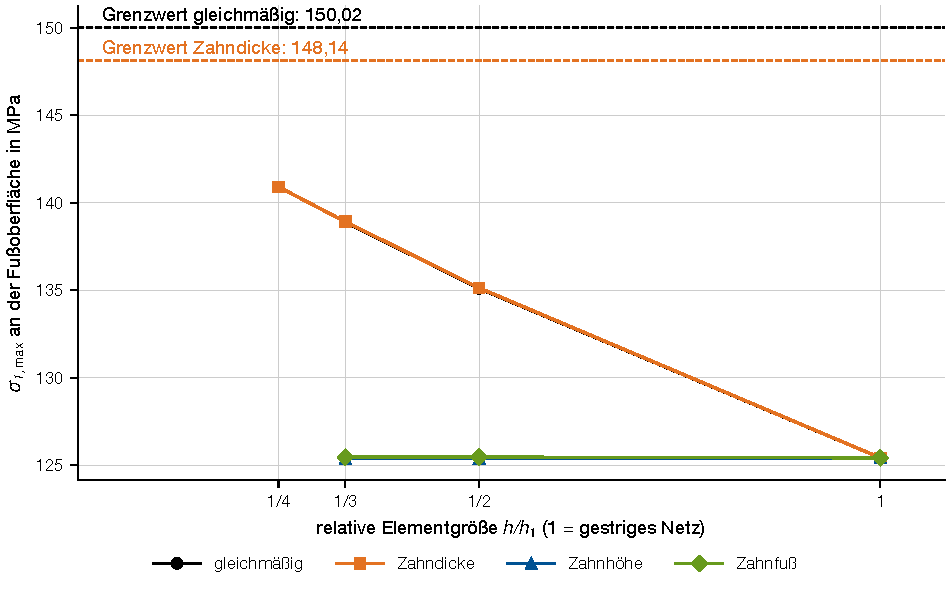
\includegraphics[width=0.8\textwidth]{kap4/konvergenz_fussspannung}
	\caption{Größte Hauptspannung an der Fußoberfläche über der relativen Elementgröße für die gleichmäßige Verfeinerung und die drei Richtungen des Netzes, Formulierung von CPE4, mit den Grenzwerten nach \eqref{eq:richardson}.}
	\label{fig:konvergenz_fussspannung}
\end{figure}
% Bildwunsch: Achsenbeschriftung "1 = Ausgangsnetz" statt "gestriges Netz"; die gleichmäßige
% Reihe mit der vierten Stufe (55 193 Knoten), damit Bild und Text denselben Grenzwert nennen.
% Bildwunsch: eine zweite Fassung der Leiter Zahndicke mit CPE4R, CPE4 und CPE4I aus den
% Abaqus-Decks (Tabelle unten), die die Unterschrift "drei Elementformulierungen" aus
% bilder.yaml einlöst; das heutige Bild zeigt nur die Formulierung von CPE4.

\figref{fig:konvergenz_fussspannung} und \tabref{tab:netzleiter} zeigen die Fußspannung. Im Ausgangsnetz beträgt sie $125{,}4$\,MPa. Eine Verfeinerung über der Zahnhöhe oder entlang der Fußrundung ändert sie um weniger als $0{,}1$\,\%. Allein die Richtung normal zur Fußoberfläche, die Sehnen der Zahndicke, hebt sie auf $135{,}1$, $138{,}9$ und $140{,}9$\,MPa. Diese Reihe konvergiert mit der Ordnung $0{,}85$ gegen $148{,}1$\,MPa, das Ausgangsnetz liegt also $15{,}4$\,\% darunter, die doppelte Zahndicke noch $8{,}8$\,\% und die vierfache $4{,}9$\,\%. Die gleichmäßige Reihe gibt über drei Stufen $150{,}0$\,MPa, mit einer vierten Stufe von 55\,193 Knoten $148{,}2$\,MPa. Der langsame Verlauf liegt an der Formulierung. Das Element hält den volumetrischen Dehnungsanteil je Element konstant, während der hydrostatische Anteil an der Kerboberfläche von null aus steil nach innen ansteigt. Die Breite der Pressungsverteilung verschiebt die Absolutwerte um etwa $5$\,\%, das Konvergenzverhalten der Reihen nicht.

% TK erledigt (Vorlage = Netz des Workbench-Referenzmodells, jetzt Ausgangsnetz; Begriffe Diskretisierung/Verfeinerungsstufe/-reihe; Workbench-Begründung und Ausgangsdiskretisierung in 3.6): Meinst du mit Vorlage das Meshbild, was ich dir mal gegeben habe? Besser spezifizieren. Gehe im Methodenteil an passender Stelle nochmal kurz in einem Satz darauf ein, dass es in der FVA Workbench mit einem fertigen Tool schwer ist, selbst Einflüsse oder Konvergenz durch Mehrfachiteration festzustellen und eigene Ansätze schwer zu integrieren sind, weswegen ich nicht drum herum gekommen bin, ein vollständiges Modell selbst aufzubauen. Auch, da bei materieller und geometrischer nicht linearität mit nachträglicher Anpassung des inp files der FVA Workbench das Konvergenzverhalten sehr schlecht war und die Konvergenzstudie und das Testen verschiedener Optionen eher schlecht mit den Tools in der Workbench möglich war. Beispielswiese Kopfkante anders aufbauen, ... und später dann auch die Fertigungstoleranzen nachträglich nach GINA anzupassen, ... ada vielleicht ein bis zwei kurze Sätze aufnehmen. Und dann kannst du hier an der Stelle auch gut sagen, das das Mesh, welches nach FVA Workbench Zahnfußspannungen konvergieren lässt bzw. ausreichend diskretisiert ist, hier als Basis Diskretisierung verwendet wurde. Verstehst du? Anstatt Dichte eher Diskretisierung verwenden. Stufen, Reihen, sehr uneinheitlich geschrieben der Text. Dem Leser ist noch nicht richtig bewusst, dass die Diskretisierung über die verschiedenen Bereiche angepasst wird. 

Für die Verformung am Zahnkopf genügt die Diskretisierung des Ausgangsnetzes. Die Verschiebung der Kopfmitte beträgt dort $203{,}8$\,\textmu m und ändert sich in keiner Reihe um mehr als $0{,}2$\,\%, die Reihe Zahndicke läuft mit der Ordnung $4{,}25$ gegen $203{,}47$\,\textmu m. Die Formänderungsenergie des Sektors ändert sich über alle Stufen um höchstens $0{,}14$\,\%, und alle drei Elementformulierungen liegen in der Kopfverschiebung innerhalb von $1{,}2$\,\% beieinander.

% Bild verfügbar, wegen des Seitenbudgets nicht eingebunden (Vorschlag: Anhang E):
% \begin{figure}[htbp]
% \centering
% 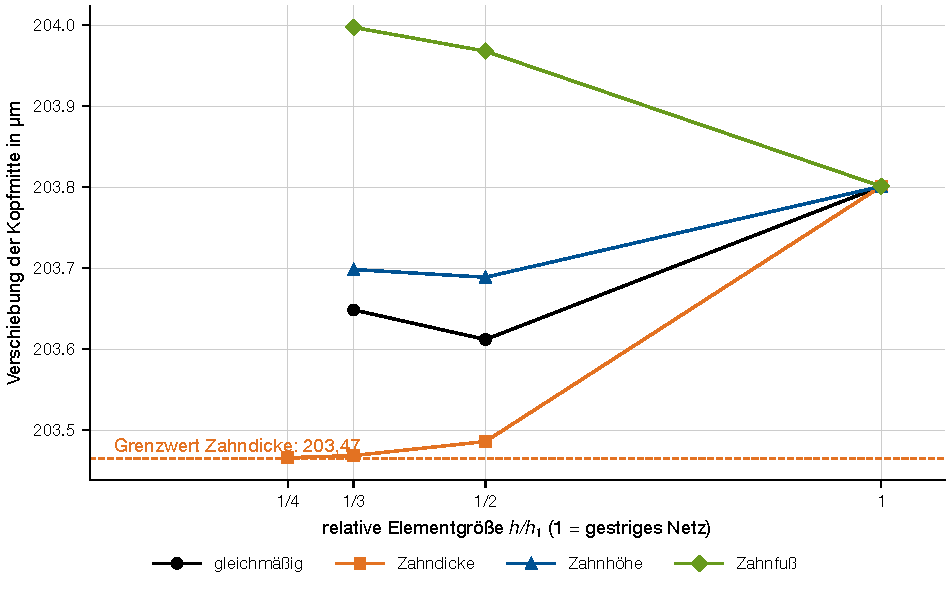
\includegraphics[width=0.8\textwidth]{kap4/konvergenz_kopfverschiebung}
% \caption{Verschiebung der Kopfmitte über der relativen Elementgröße für die gleichmäßige Verfeinerung und die drei Richtungen des Netzes, Formulierung von CPE4.}
% \label{fig:konvergenz_kopfverschiebung}
% \end{figure}

\begin{table}[htbp]
	\centering
	\caption{Verfeinerungsreihe über der Zahndicke am ebenen Radsektor, gerechnet auf der Abaqus-Vollversion: größte Hauptspannung an der Fußoberfläche und Verschiebung der Kopfmitte je Elementformulierung, Grenzwert und Ordnung nach \eqref{eq:richardson}.}
	\label{tab:netzleiter}
	\begin{tabular}{lllllll}
		\hline
		Elemente über der & Knoten je & \multicolumn{3}{l}{$\sigma_{\mathrm{1}}$ am Fuß in MPa} & \multicolumn{2}{l}{Kopfmitte in \textmu m}                                      \\
		Zahndicke         & Schicht   & CPE4R                                                   & CPE4                                       & CPE4I      & CPE4      & CPE4I     \\
		\hline
		\arrayrulecolor{black!30}
		10                & 3\,719    & $114{,}85$                                              & $125{,}42$                                 & $141{,}60$ & $203{,}8$ & $202{,}0$ \\
		\hline
		20                & 7\,021    & $127{,}94$                                              & $135{,}13$                                 & $147{,}61$ & $203{,}5$ & $203{,}1$ \\
		\hline
		30                & 10\,323   & $133{,}57$                                              & $138{,}91$                                 & $148{,}50$ & $203{,}5$ & $203{,}3$ \\
		\hline
		40                & 13\,625   & $136{,}69$                                              & $140{,}90$                                 & $148{,}62$ & $203{,}5$ & $203{,}4$ \\
		\hline
		Grenzwert         &           & $150{,}5$                                               & $148{,}1$                                  & $148{,}7$  & $203{,}5$ & $203{,}6$ \\
		\hline
		Ordnung           &           & $0{,}71$                                                & $0{,}85$                                   & $4{,}63$   & $4{,}25$  & $1{,}8$   \\
		\arrayrulecolor{black}
		\hline
	\end{tabular}
\end{table}

Die Elementformulierung wiegt so schwer wie die Diskretisierung (vgl. \tabref{tab:netzleiter}). Mit reduzierter Integration, dem ebenen Gegenstück des C3D8R im Referenznetz, liegt der Knotenwert im Ausgangsnetz bei $114{,}9$\,MPa und damit rund $23$\,\% unter dem Grenzwert. Die Hourglass-Energie bleibt dabei unter $0{,}04$\,\% der Formänderungsenergie und ist nach der Energiebilanz unkritisch \cite[S.~428]{Sto18}. Mit inkompatiblen Moden liefert dasselbe Netz $141{,}6$\,MPa und damit $4{,}7$\,\% unter dem Grenzwert, die doppelte Zahndicke $147{,}6$\,MPa mit $0{,}7$\,\%, und die Reihe konvergiert mit der Ordnung $4{,}6$. Alle drei Formulierungen weisen auf denselben Grenzwert zwischen $148$ und $149$\,MPa. Für die Wahl der Diskretisierung wurde eine Verfeinerungsreihe aus Zahndicke und Fußschichten mit diesem Element gerechnet und nach \eqref{eq:richardson} über alle Stufen ausgeglichen. Die Toleranz betrug $2$\,\% für die Fußspannung und $1$\,\% für die Kopfverschiebung. Die Stufe mit 14 Elementen über der Zahndicke und 4 Fußschichten liegt $1{,}8$\,\% unter dem Grenzwert, die Stufe mit 20 und 6 noch $0{,}7$\,\%. Die übrigen Anzahlen wurden einzeln vergröbert, solange beide Größen in der Toleranz blieben, nur die Zahnhöhe behielt ihre 18 Elemente, weil der Kontakt drei Elemente je Hertzscher Halbbreite verlangt. Das empfohlene Netz hat 18 Elemente über der Zahnhöhe und eines am Kopfkantenbruch, 60 am Zahnfuß, 14 über der Zahndicke mit 4 Fußschichten und 4 Kranzringe. Mit 3\,890 Knoten je Schicht liegt seine Fußspannung $1{,}9$\,\% unter dem Grenzwert.

Die ersten Stellungsdateien mit C3D8I und geometrisch nichtlinearer Rechnung brachen im Schritt mit $12$\,Nm ab. Warnungen negativer Eigenwerte der Systemmatrix erschienen ab dem ersten Lastinkrement und bei allen drei Kontaktformulierungen gleich. Ein Elementtest am Grobmodell der Learning Edition mit einem Zahn, zwei Schichten und 414 Knoten trennte die Ursache. Mit C3D8I und dem Schalter NLGEOM=YES erscheinen 29 Warnungen ab dem Schritt mit $8$\,Nm, Inkrement 1, während dasselbe Modell mit C3D8 oder C3D8R geometrisch nichtlinear ohne eine einzige Warnung rechnet. Die Elementdokumentation von Abaqus beschränkt Elemente mit inkompatiblen Moden auf kleine Druckdehnungen \cite{AbaqusSolid25}. Am Pilotnetz mit 20 Schichten und 81\,690 Knoten laufen beide C3D8-Dateien alle vier Schritte ohne negativen Eigenwert durch, in $140$ und $161$\,s gegen $173$\,s für C3D8I. Die geometrische Nichtlinearität ändert bis $16$\,Nm das Stützmoment um $0{,}1$\,\%, den Verdrehwinkel des Ritzels um $0{,}5$\,\% und die größte Pressung um $0{,}7$\,\%. Der Wechsel von C3D8I auf C3D8 ändert diese Größen um weniger als $1$\,\%.

Daraus folgt die Regel je Werkstoffstufe. Die elastischen Stufen W1 und W3 werden geometrisch linear mit C3D8I gerechnet, weil ein lineares Problem linear gerechnet wird \cite[S.~474]{Sto18} und die Fußspannung dort innerhalb von $2$\,\% am Grenzwert liegt. Die elastisch-plastischen Stufen W2 und W4 brauchen die geometrisch nichtlineare Rechnung, da sich Kunststoffe schon bei geringen Lasten plastisch verformen und die geometrische Nichtlinearität mit der Dehnung wächst \cite[S.~2, 52, 474]{Sto18}. Sie werden mit C3D8 auf demselben Netz gerechnet, Elementnummern und Faserorientierung bleiben erhalten. Die Verfeinerungsreihe mit der Formulierung von C3D8 konvergiert an der Fußoberfläche nur mit der Ordnung $0{,}81$ und erreicht auf keiner Stufe $2$\,\%. Bei 14 Elementen und 4 Fußschichten liegt sie $12{,}0$\,\% unter dem Grenzwert, bei 40 und 12 mit 286\,000 Knoten im Volumen noch $4{,}9$\,\%. Fußspannungen einer C3D8-Stufe sind deshalb mit denen einer C3D8I-Stufe nur auf gleichem Elementtyp oder gegen den extrapolierten Grenzwert vergleichbar.

% TK erledigt (Leiter → Verfeinerungsreihe/-stufe): Leiter ist ein komischer Ausdruck dafür. Bitte an der Stelle und anderen entsprechend anderen Begriff verwenden

Das ebene Modell prüft die Zahl der Schichten über der Zahnbreite nicht. Volumendecks der Ausgangsdiskretisierung mit 20, 40 und 80 Schichten, gerechnet auf der Vollversion mit C3D8I, geben in der Radmitte $204{,}87$, $204{,}93$ und $204{,}95$\,\textmu m sowie $143{,}49$, $143{,}53$ und $143{,}55$\,MPa. Nur der Wert unmittelbar an der Stirnfläche fällt mit feinerer Teilung weiter von $108{,}3$ auf $96{,}8$\,MPa, er gehört zum freien Rand und ist keine Zielgröße. Gegenüber dem Volumenmodell nimmt der ebene Dehnungszustand das Rad in der Radmitte um $1{,}4$\,\% zu steif. Die Pilotläufe der Stellungsdatei mit 40 und 80 Schichten ließen Momente und Verdrehwinkel des Ritzels auf vier Stellen unverändert und hoben die größte Pressung um $1$\,\%. Eingefroren wurde deshalb das Netz mit 20 Schichten in der empfohlenen Diskretisierung, mit fünf Kranzringen bis zur Bohrung von $33$\,mm, dem Innendurchmesser des Kunststoffbereichs am realen Rad. Das eingefrorene Netz mit Ringkörper hat 82\,425 Knoten, der Taschenkörper folgt in \secref{sec:stufen_raten_koerper}, die Tabellen aller Reihen stehen in \anhref{sec:anhang_e}.

% Bild verfügbar, wegen des Seitenbudgets nicht eingebunden (Vorschlag: Anhang E):
% \begin{figure}[htbp]
% \centering
% 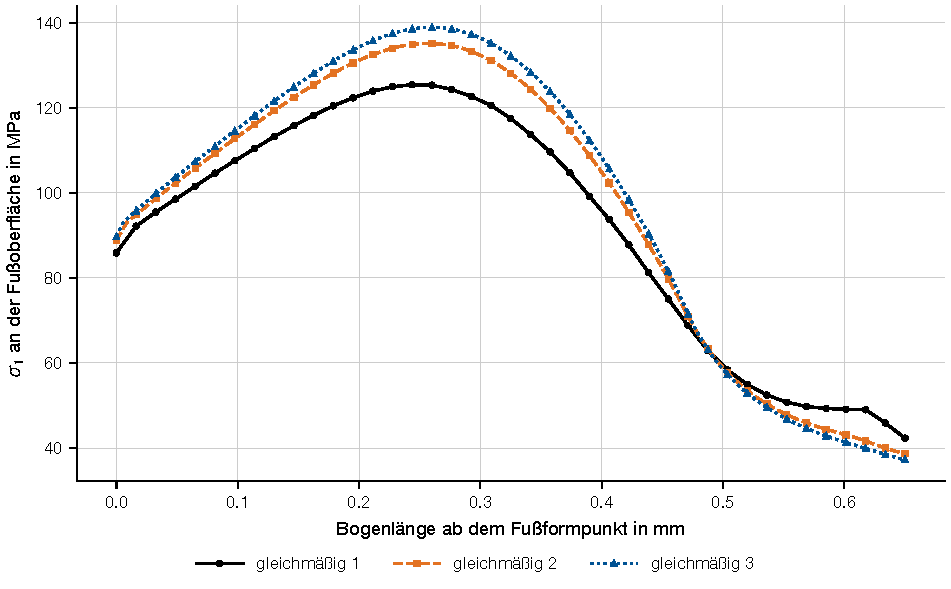
\includegraphics[width=0.8\textwidth]{kap4/fussspannung_verlauf_eben}
% \caption{Verlauf der größten Hauptspannung entlang der Fußrundung der belasteten Flanke für die gleichmäßigen Stufen 1 bis 3 im ebenen Modell.}
% \label{fig:fussspannung_verlauf_eben}
% \end{figure}

% Herkunft:
% Absatz 1 (Vorgehen, Löser, Prüfung): 20_code/00_development_documentation/fe_mesh_convergence.md
%   Abschnitt 2 (Stommel 7.7.1 S. 424, 7.7.3 S. 433, 8.2.2 S. 465; ebener Sektor als Auszugsnetz;
%   Löser; Prüfung Learning Edition 7e-5) und Abschnitt 5a (Vollversion: CPE4 alle gedruckten
%   Stellen, CPE4I 0,01 MPa und 0,01 µm); 80_output/fe/kst_e/convergence/verification.md
%   (859 Knoten, Tabelle); architecture_decisions.md ADR-116 Punkt 12.
% Absatz 2 (Lastfall, Größen, Reihen, Formel): fe_mesh_convergence.md Abschnitt 2 (Last, Hertz nach
%   Nie19 Tab. 13.1, E = 2282 MPa, ν = 0,30, Fesselung, bewertete Größen, Reihen, Richardson nach
%   Bathe und Dahmen/Reusken) und Abschnitt 1 Tabelle (Vorlage 20 / 80 / 10);
%   Bild load_case.png (F' = 43,66 N/mm, b_H = 0,322 mm, p_0 = 86,4 MPa).
% Absatz 3 (Fußspannung): fe_mesh_convergence.md Abschnitt 3 Tabelle und Extrapolation (Zahndicke
%   p = 0,85 gegen 148,1; Fehler −15,4 / −8,8 / −6,2 / −4,9 %; gleichmäßig vier Stufen p = 0,84
%   gegen 148,2 mit 55 193 Knoten; Lastbreite etwa 5 %), Abschnitt 4 Punkt 2 (Ursache, erste
%   Schicht 0,02 mm); 80_output/fe/kst_e/bilder_V2/convergence/convergence.md (gleichmäßig drei
%   Stufen p = 0,72 gegen 150,0; Zahnhöhe und Zahnfuß ≤ 0,03 %); Bild convergence_root_stress.png.
% Absatz 4 (Kopfverschiebung, Energie): bilder_V2/convergence/convergence.md Extrapolation Reihe
%   Zahndicke (u Kopfmitte p = 4,25 gegen 203,465 µm); fe_mesh_convergence.md Abschnitt 3
%   (≤ 0,2 %, U ≤ 0,14 %) und Abschnitt 4 Punkt 1 (drei Formulierungen innerhalb 1,2 %).
% Tabelle: 80_output/fe/kst_e/full_licence_result/comparison.md (ebene Decks base/t2/t3/t4 je
%   CPE4R/CPE4/CPE4I; Grenzwerte 150,47 (0,71), 148,13 (0,85), 148,66 (4,63)); Kopfmitte CPE4
%   Grenzwert und Ordnung aus bilder_V2/convergence/convergence.md (203,465, p = 4,25), CPE4I
%   Grenzwert 203,6 µm (p = 1,8) aus fe_mesh_convergence.md Abschnitt 3 (eigener Löser).
% Absatz 5 (Elementtyp, Empfehlung): fe_mesh_convergence.md Abschnitt 4 Punkte 3 und 4, Abschnitt
%   5a (Hourglass < 0,04 %), Abschnitt 5b (Leiter 14/4 −1,82 %, 20/6 −0,72 %; Reduktion; Zahnhöhe
%   Untergrenze 19; Empfehlung 18 + 1 / 60 / 14 / 4 / 4 / 2, 3 890 Knoten, −1,9 %);
%   80_output/fe/kst_e/recommendation/recommendation.md; ADR-116 Punkte 13 bis 15.
% Absatz 6 (Nichtlinearität, Elementtest, Bestätigung): fe_mesh_convergence.md Abschnitt 5c;
%   80_output/fe/kst_e/le_tests/element_nlgeom/ELEMENT_TEST.md (414 Knoten, 29 Warnungen ab 8 Nm
%   Inkrement 1; das Tagebuch fe_simulation_log.md zählt für denselben Lauf 30 negative
%   Eigenwerte); ADR-116 Punkte 18 und 20 (140 s / 161 s / 173 s; das Tagebuch nennt für
%   pilot_20layers_c3d8_variants_gerechnet 157 s und 174 s Wandzeit); known_limits.md FE-14.
% Absatz 7 (Regel je Stufe): ADR-116 Punkte 19 (b), 19 (c) und 21 (Stommel S. 2, 52, 474);
%   fe_mesh_convergence.md Abschnitt 5c Tabelle (C3D8-Leiter Ordnung 0,81, −12,0 / −8,8 / −4,9 %,
%   286 125 Knoten bei 20 Schichten); known_limits.md FE-10.
% Absatz 8 (Schichten, Bohrung, Einfrieren): full_licence_result/comparison.md Volumendecks
%   (C3D8I 20/40/80 Schichten); fe_mesh_convergence.md Abschnitt 5a (Stirnfläche 108 → 97 MPa,
%   ebener Zustand 1,4 % zu steif) und Abschnitt 6; ADR-116 Punkt 22 (Piloten 40/80 Schichten,
%   Bohrung 16,5 mm Radius = 33 mm, Stahleinleger als Fesselung, 82 425 Knoten);
%   known_limits.md FE-08 und FE-09.

\section{Eingriffsauflösung und Kopfkante}
\label{sec:kopfkante}

Die Stellungen des Eingriffs werden als getrennte statische Rechnungen über dem Eingriffsweg aufgereiht (vgl. \secref{sec:fe_modell}). Wie dicht sie liegen müssen, wurde mit 60 Stellungen je Teilung am Ringkörper unter W1 bestimmt. Von 133 Stellungen liefen 122 durch, elf brachen ab. Bei $16$\,Nm trägt der nachfolgende Zahn durch die Verformung bereits $1{,}65$\,mm vor A. Die Kopfkante des Ritzels bleibt am auslaufenden Zahn $1{,}5$\,mm hinter E im Kontakt. Die größte Fußspannung des Rades liegt deshalb im Bereich des Normpunktes C und nicht bei B. Bei $16$\,Nm halten 30 Stellungen je Teilung die Größtwerte innerhalb $0{,}15$\,\% und 20 innerhalb $1{,}6$\,\%, letzteres an einem Knick von $|\sigma_{\mathrm{3}}|$. Mit 20 je Teilung wandern die Maxima von Verformung und Fußspannung um weniger als $0{,}05$\,mm. Bei $8$\,Nm sind die Maxima Knicke an den Übergängen der Zahl tragender Paare. Dort verfehlt das Gitter mit 30 je Teilung einen Größtwert um $1{,}7$\,\%, das Gitter mit 20 trifft ihn.

Für die Serie aller vier Werkstoffstufen wurden 30 Stellungen je Teilung und ein Rand von einer Teilung vor A und hinter E gewählt. Ein Rand von einer halben Teilung war in einem Vorlauf mit W4 zu kurz, die äußeren Zähne trugen an den Gitterenden noch $10$\,\% und $30$\,\% der Zahnkraft. In der Serie trägt der mittlere Zahn bis zu $0{,}60$ Teilungen vor A und bis zu $0{,}48$ Teilungen hinter E, mit Moment und Plastizität wachsend. Innerhalb dieses Gitters verändern 15 Stellungen je Teilung die Größtwerte um höchstens $2{,}9$\,\% bei W3 und $16$\,Nm, 10 je Teilung um $5{,}5$\,\%.

Alle elf Abbrüche der Studie liegen an drei Wegstellen je Teilung. Dort sitzt die scharfe Kopfkante des starren Ritzels auf einer Knotenreihe der Flanke des auslaufenden Zahns hinter E. Die Knotenreihen liegen auf den Radien $25{,}698$, $25{,}800$ und $25{,}901$\,mm der Radflanke, also $0{,}1$\,mm auseinander. Der Knoten auf dem Knick meldet einen zu großen Durchdringungsfehler, das Inkrement wird bis auf $10^{-6}$ verkürzt, und die Rechnung endet. Weder eine Strafsteifigkeit statt der Lagrange-Multiplikatoren noch erhöhte Iterationsgrenzen helfen. Ursache ist die Mehrdeutigkeit der Flächennormalen an einer scharfen Ecke, der Löser wählt einen der beiden Zweige zufällig. Eine Rundung von $0{,}05$\,mm, kleiner als der Reihenabstand, verlagert den Abbruch auf die Nachbarstellung. Erst die Rundung $0{,}1$\,mm mit 12 Facetten rechnet alle geprüften Stellungen in sechs Inkrementen je Schritt ohne Warnung durch. Eine berührende konvexe Kante braucht demnach mindestens den Reihenabstand der Gegenfläche in Gleitrichtung als Radius. In der Serie brach mit dieser Kante noch eine von 396 Rechnungen ab.

Gegenüber der scharfen Kante verändert die Rundung das Ergebnis nur dort, wo die Kopfkante des Ritzels Last trägt. An 68 gemeinsamen Stellungen von Studie und Serie unter W1 steigt der Verdrehwinkel des Ritzels an B und E um $5{,}3$\,\% bis $6{,}8$\,\%. Der Kontaktdruck an der Kante fällt dort um $8{,}0$\,\% bis $10{,}8$\,\%, die Zugspannung $\sigma_{\mathrm{1}}$ um $4{,}7$\,\% bis $8{,}7$\,\%. An A, C und D bleiben alle Größen innerhalb $0{,}3$\,\%. Der Abschnitt des Wälzwegs um B und E, in dem die Rundung wirkt, ist etwa $0{,}3$\,mm lang. Die Größtwerte über dem ganzen Weg ändern sich bei $12$ und $16$\,Nm um höchstens $2{,}5$\,\%, bei $8$\,Nm um bis zu $4{,}9$\,\%.

Ob diese Empfindlichkeit an der Kante oder am Netz der Radflanke hängt, klärte ein Nachtlauf mit feinerer Flanke. Die Zahl der Reihen über der Zahnhöhe, der einzige Hebel für den Reihenabstand in Gleitrichtung, stieg von 18 auf 36 und 54. Der Abstand sank von etwa $0{,}1$\,mm auf etwa $0{,}05$ und $0{,}033$\,mm. Jedes Netz wurde mit Ritzelkanten von $0{,}1$, $0{,}05$ und $0{,}02$\,mm gepaart, W1 bei QS an den Normpunkten A bis E, die Kante $0{,}05$\,mm zusätzlich mit W2. \tabref{tab:netz_rundung} stellt die Änderungen gegen die Serie bei $12$\,Nm zusammen, dem Schritt, in dem alle Rechnungen durchliefen. Bei $16$\,Nm bricht W1 mit der Kante $0{,}05$\,mm auf 36 Reihen an B und E und auf 54 Reihen an E nach dem Muster der Studie ab. Mit $0{,}02$\,mm laufen alle fünf Stellungen auf beiden Netzen durch, ebenso jede Rechnung mit W2. Der Abbruch hängt damit am Verhältnis von Facettenlänge zu Reihenabstand und nicht am Radius allein.

\begin{table}[htbp]
    \caption{Netzeffekt gegen Rundungseffekt: Änderung der Werte an den Normpunkten gegen das Netz mit 18 Reihen über der Zahnhöhe und der Ritzelkante $0{,}1$\,mm, Ringkörper, W1, quasistatische Karte, $12$\,Nm. Verdrehwinkel des Ritzels, größte Zugspannung $\sigma_{\mathrm{1}}$ der Fußrundung und größter Kontaktdruck $p$ unter der Kante, alle Angaben in \%.}
    \label{tab:netz_rundung}
    \centering
    \footnotesize
    \setlength{\tabcolsep}{3pt}
    \begin{tabular}{lllllllll}
        Reihen & Kante in mm & Verdrehwinkel C & Verdrehwinkel B & Verdrehwinkel E & $\sigma_{\mathrm{1}}$ C & $\sigma_{\mathrm{1}}$ B & $\sigma_{\mathrm{1}}$ E & $p$ B     \\
        \hline
        \arrayrulecolor{black!30}
        36     & $0{,}1$     & $-1{,}6$  & $-2{,}0$  & $-2{,}2$  & $-1{,}7$                & $+3{,}7$                & $+0{,}9$                & $+50{,}6$ \\
        \hline
        36     & $0{,}05$    & $-3{,}5$  & $-4{,}9$  & $-5{,}1$  & $-3{,}3$                & $+7{,}6$                & $+3{,}8$                & $+59{,}9$ \\
        \hline
        36     & $0{,}02$    & $-3{,}5$  & $-5{,}0$  & $-5{,}3$  & $-3{,}3$                & $+9{,}3$                & $+5{,}9$                & $+59{,}9$ \\
        \hline
        54     & $0{,}1$     & $-1{,}9$  & $-2{,}6$  & $-2{,}8$  & $-1{,}6$                & $+5{,}5$                & $+2{,}6$                & $+93{,}6$ \\
        \hline
        54     & $0{,}05$    & $-3{,}8$  & $-4{,}8$  & $-5{,}0$  & $-3{,}9$                & $+8{,}1$                & $+4{,}1$                & $+97{,}0$ \\
        \hline
        54     & $0{,}02$    & $-4{,}4$  & $-4{,}9$  & $-5{,}2$  & $-4{,}3$                & $+9{,}3$                & $+5{,}8$                & $+96{,}4$ \\
        \hline
        \arrayrulecolor{black}
    \end{tabular}
\end{table}

% TK erledigt (Ritzeldrehung in 3.6 definiert: Verdrehwinkel bis zum Gleichgewicht aus Zahnbiegung und Kontakt, nicht das Flankenspiel; zum Kantendruck siehe den neuen Absatz am Ende): Drehung hatten wir glaube auch schonmal gesprochen, dass du eigentlich das Verdrehwinkelspiel meinst oder meinst du hier was anderes? Bitte nochmal besser spezifizieren, was du mit Drehung aussagen möchtest. Und wir haben ja jetzt mit 0,1 Rundung weitergearbeitet, aber ich finde es krass, dass bei 54 Reihen und 0,02er Rundung alles durchgelaufen ist und der Kontaktdruck +96 % hat. Das ist ja verrückt.

Der Netzeffekt allein zeigt sich mit der Kante $0{,}1$\,mm auf 36 und 54 statt 18 Reihen. Er senkt den Verdrehwinkel des Ritzels an A, C und D um bis zu $1{,}9$\,\% und an B und E um $1{,}8$\,\% bis $3{,}2$\,\%. An A, C und D bleibt die Zugspannung $\sigma_{\mathrm{1}}$ innerhalb $3$\,\%, an B steigt sie um $2{,}2$\,\% bis $5{,}5$\,\%. Der größte Kontaktdruck unter der Kante wächst dagegen mit jeder Verfeinerung weiter. An B steigt er mit 36 Reihen um $51$ bis $60$\,\% und mit 54 Reihen um $94$ bis $97$\,\% (\tabref{tab:netz_rundung}), an E in ähnlicher Höhe. Ein konvergierter Wert existiert nicht. Mit der aufgelösten scharfen Kante, $0{,}02$\,mm auf 54 Reihen, dreht das Ritzel gegenüber der Serie um $2{,}0$\,\% bis $4{,}4$\,\% weniger an A, C und D. An B und E sind es $4{,}5$\,\% bis $5{,}9$\,\% weniger. Die Zugspannung liegt an C um $2{,}4$\,\% bis $4{,}3$\,\% tiefer, an B um $7{,}5$\,\% bis $9{,}4$\,\% und an E um $4{,}7$\,\% bis $6{,}0$\,\% höher.

% TK erledigt (Text auf die Werte an B der Tabelle gebracht, E nur qualitativ): in der Tabelle stehen keine 103 % sondern 96,4 %. Bitte Zahlen im Text passend zu den Tabellen oder irgendwas ist durcheinander gekommen.

Die reale Kante des Prüfstandsritzels 95912 wurde an drei Zähnen im Konturscan aufgenommen. An jede Kante wurden ein tangentialer Bogen vom Radius $\rho$ und eine symmetrische Fase mit dem Schenkel $c$ gefittet. \figref{fig:kopfkante_95912} zeigt Zahn 18 mit Bogenradien von $0{,}004$ bis $0{,}008$\,mm bei einer Restabweichung von $0{,}9$ bis $1{,}3$\,µm. Zahn 1 liegt im Mittel bei $0{,}004$\,mm. Mikroskopaufnahmen der drei Zahnköpfe zeigen die gedrehte Kopffläche und die gewälzfräste Flanke an einer Kante ohne Fasenfacette und ohne sichtbares Rundungsband. Daraus folgt nur ein Radius unter etwa $20$\,µm. Auch das ältere Ritzel 86481 trägt mit einem Bogen von im Mittel $0{,}008$\,mm eine scharfe Kante.

\begin{figure}[htbp]
    \centering
    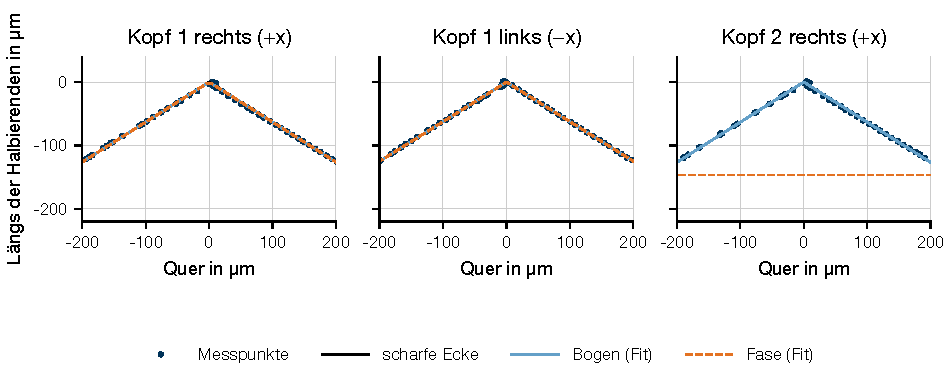
\includegraphics[width=0.8\textwidth]{kap4/kopfkante_95912}
    \caption{Kopfkante des Prüfstandsritzels 95912 im Konturscan, Zahn 18, rechte und linke Kante des ersten Zahnkopfs: Messpunkte, Lage der scharfen Ecke, tangentialer Bogen und symmetrische Fase als Fit, die Bogenradien stehen im Text.}
    \label{fig:kopfkante_95912}
\end{figure}

% TK (folgt mit Paket B4, Bild wird neu gezeichnet): Bitte Kopf 2 rausnehmen. Da ist eh was falsch mit einer Geraden als Fasenfit und Kopf 1 rechts und links reicht.

Die Rundung $0{,}1$\,mm mit 12 Facetten ist damit eine Modellwahl und keine Eigenschaft des Teils. Dass trotz der Verdopplung des Kantendrucks mit dieser Rundung weitergerechnet wurde, hat drei Gründe. Der Druck unter einer nahezu scharfen Kante ist ein Linienkontakt ohne konvergierenden Wert, jede Verfeinerung hebt die Spitze weiter. Er ist deshalb keine Bemessungsgröße dieser Arbeit und wird in den Ergebniskapiteln als netz- und kantenabhängige Größe geführt. Die Zielgrößen am Fuß ändern sich mit Kante und Reihenzahl an B und E um höchstens $9{,}4$\,\% in $\sigma_{\mathrm{1}}$ und rund $5$\,\% im Verdrehwinkel des Ritzels. An den übrigen Normpunkten und an den Größtwerten sind es wenige Prozent. Dazu kommt, dass die reale Kante mit einem Radius unter $20$\,µm schärfer ist als jedes Modell. Sie arbeitet sich im Versuch in die Radflanke ein (\secref{sec:schadensbilder}), so dass der Kantendruck des unverschlissenen Modells das Teil ohnehin nicht beschreibt. Ein Modell mit scharfer Kante bräuchte $0{,}02$\,mm auf mindestens 36 Reihen.

% TK erledigt (drei Gründe im Text; Mapping gab es nur für das 18-Reihen-Netz, die 36/54-Piloten liefen mit W1/W2): Wenn das im Kontaktdrcuk Abweichungen von 100 % waren grob, dann bitte hier noch eine bessere erklärung, warum doch einfach mit der 0,1er Rundung weiter gearbeitet wurde, da wir ja das mapping auf die feineren Reihen durchgeführt hatten. 

% Herkunft:
% Absatz 1 (Studie 60 je Teilung): ADR-116 Punkt 36 (architecture_decisions.md, Amendment 2026-10-09);
%   Teilgitter-Zahlen aus 80_output/fe/kst_e/study_20layers_bore33_60perpitch_gerechnet/path_report.md
%   (LOAD_16NM: 30 je Teilung s1_max −0,14 %, 20 je Teilung s3_min −1,59 % und Versatz ≤ 0,035 mm
%   ausser p_max +0,117 mm bei −0,03 %, 15 je Teilung s3_min −2,12 %, 10 je Teilung s3_min −2,47 %;
%   LOAD_8NM: 30 je Teilung s3_min −1,74 %, 20 je Teilung 0,00 %).
% Absatz 2 (Serie, Rand): series_..._30perpitch_margin1_qs_gerechnet/analyse/analyse.md Kopf (396 Dateien,
%   30 je Teilung, Rand 1,00, 99 Stellungen je Stufe) und Abschnitt 6 (15 je Teilung +2,9 % W3 16 Nm, 10 je Teilung +5,5 %);
%   ADR-116 Punkt 41 (Rand 0,5 Teilung zu kurz, 10 und 30 % der Zahnkraft) und Punkt 47 (a)
%   (0,47 bis 0,60 vor A, 0,35 bis 0,48 hinter E).
% Absatz 3 (Abbrüche, Rundung 0,1 mm mit 12 Facetten): ADR-116 Punkte 37 und 43; known_limits.md FE-19
%   (zwei Arten, Versatz 0,025 mm, Zweige der Normalen, Regel Reihenabstand, 1 von 396 pos_073);
%   series analyse.md Abschnitt 1 (pos_073_W1_QS bei 16 Nm, 3,838 mm ab A, r 25,800 mm).
% Absatz 4 (scharf gegen gerundet): series analyse.md Abschnitt 5 (68 Stellungen, Tabellen 8/12/16 Nm:
%   Drehung B +6,7/+5,6/+5,3, E +6,8/+5,9/+5,4; Druck B −9,9/−10,8/−9,1, E −9,0/−9,5/−8,0;
%   σ1 B −7,5/−8,3/−8,7, E −4,7/−5,3/−5,7; A, C, D höchstens +0,3 % (Druck an C);
%   Maxima 8 Nm bis +4,9 %, 12 Nm bis +1,6 %, 16 Nm bis +2,5 %); ADR-116 Punkt 47 (c) (Fenster 0,3 mm);
%   known_limits.md FE-17. Abweichung: ADR nennt "Maxima innerhalb 2,5 %", die Tabelle bei 8 Nm +4,6 % (σ1)
%   und +4,9 % (|σ3|); der Text folgt der Tabelle.
% Absatz 5 und Tabelle (Nachtlauf, Netz gegen Rundung): ADR-116 Punkt 50 mit Amendment und Outcome
%   (18/36/54 Reihen, Abstände, Abbrüche); fe_simulation_notes.yaml outcome der sechs Ordner
%   pilot_20layers_bore33_hoehe{36,54}_round0p{02,05,1}f12_*_qs_AtoE_gerechnet; Tabelle: Abschnitt 5
%   (Vergleich mit der Serie) der sechs analyse.md, Block 12 Nm, Spalten C, B, E.
% Absatz 6 (Netzeffekt, aufgelöste Kante): dieselben sechs analyse.md, Abschnitt 5, Blöcke 8/12/16 Nm,
%   Spannen über die drei Schritte selbst gebildet (Netzeffekt 0,1 mm: Drehung A/C/D +0,1 bis −1,9 %,
%   B/E −1,8 bis −3,2 %, σ1 A/C/D −3,0 bis +0,2 %, B +2,2 bis +5,5 %; Druck B/E +48,3 bis +57,2 % (36)
%   und +86,8 bis +102,8 % (54); aufgelöste Kante hoehe54_round0p02: Drehung A/C/D −2,0 bis −4,4 %,
%   B/E −4,5 bis −5,9 %, σ1 C −2,4 bis −4,3 %, B +7,5 bis +9,4 %, E +4,7 bis +6,0 %); W2 gegen W1
%   Kontaktdruck an B/E (−32,7/−45,0 % auf 36 Reihen, −37,5/−51,3/−58,3 % auf 54; Abschnitt 3 der
%   round0p05-Ordner) aus dem Text gestrichen, Stoff für 4.3. Abweichung: ADR-116 Punkt 50 nennt σ1 an A, C, D "innerhalb ±1 %" und
%   Drehung A/C/D "−2,6 bis −3,5 %"; die 12-Nm- und 16-Nm-Blöcke reichen weiter (σ1 A/D 16 Nm −3,0/−2,8 %,
%   Drehung C 12 Nm −4,4 %); der Text folgt den Tabellen.
% Absatz 7 und Bild (reale Kante): 80_output/messungen/konturscan/pinion/bericht.md Kopf (Fit Bogen/Fase),
%   Tabelle je Scan (95912_Z01 ρ 0,004, Z18 ρ 0,006; Z36 ρ 0,091 wegen eines als Kopffläche erkannten
%   Laufs 0,28 mm unter den anderen nicht genannt, ADR-117 Punkt 4) und
%   je Teil (86481 ρ Mittel 0,008, max 0,018); SVG kopfkante_95912_95912_Z18 (ρ 0,008/0,004/0,005 mm,
%   RMS 1,3/0,9/1,3 µm); ADR-117 Amendment 2026-10-12 Punkt 4 (Maschinenhöhe 87,57 bis 87,62 mm,
%   Bogen 0,002 bis 0,008 mm, Mikroskop F4092 Z1/Z18/Z36, Maßbalken 200 µm, "unter etwa 20 µm",
%   Rücknahme 25 bis 27 µm gegen fKo −22,7/−23,4 µm). Hinweis: Die Vorgabe "Kopfrücknahme nur beim
%   älteren Ritzel 86481" steht gegen bericht.md (Gerade am Nennkopfkreis 86481 20,8 µm, 95912 25,9 µm)
%   und ADR-117; deshalb der Platzhalter. Die Fasen-Schenkel der bericht.md-Tabelle (0,062/0,093 mm)
%   weichen von ADR-117 (0,001 bis 0,004 mm) und vom SVG (0,004/0,002/0,274 mm) ab; der Text nennt
%   deshalb nur die Bogenradien.
% Absatz 8 (Folgerung): ADR-116 Punkt 50 Outcome (Decision) und Punkt 43; known_limits.md FE-17 (Modellparameter).
% Bildwunsch: 80_output/fe/kst_e/series_20layers_bore33_round0p1f12_30perpitch_margin1_qs_gerechnet/analyse/vergleich_referenz_LOAD_16NM.svg,
%   Rundung 0,1 mm gegen scharfe Kante über dem Eingriffsweg (Fenster um B und E; Legende ohne "Serie"/"Referenz").
% Bildwunsch: Kurven der 60-je-Teilung-Studie mit den Teilgittern 30/20/15/10 (im Studienordner liegen nur mesh_*.png,
%   bilder_V2/study_* nicht gefunden; neu zu zeichnen aus den Stellungsdateien des Studienordners).
% Bildwunsch: 80_output/fe/kst_e/pilot_20layers_bore33_hoehe54_round0p02f12_w1_qs_AtoE_gerechnet/analyse/vergleich_referenz_LOAD_16NM.svg
%   (oder ein Sammelbild der sechs Nachtlauf-Ordner als Marker an A bis E), Netzeffekt gegen Rundungseffekt.
% Bildwunsch: Mikroskopaufnahme F4092 95912 Z18 (Inventar, Art microscope) als Ergänzung zum Konturscan der Kante.

\section{Werkstoffstufen, Dehnraten und Radkörper}
\label{sec:stufen_raten_koerper}

Dieser Abschnitt trennt am Sektormodell aus \secref{sec:fe_modell} die Einflüsse der Werkstoffstufe, der Dehnrate der Werkstoffkarte und des Radkörpers. Grundlage ist die Serie des Ringkörpers mit 99 Stellungen von einer Teilung vor A bis einer Teilung hinter E mit der quasistatischen Karte (QS). Gerechnet wurden die vier Stufen W1 (linear-elastisch, isotrop), W2 (elastisch-plastisch, isotrop), W3 (linear-elastisch, anisotrop) und W4 (elastisch-plastisch, anisotrop) nach der Abstufung von \cite{Sto18}, und 395 der 396 Rechnungen liefen vollständig durch (vgl. \secref{sec:kopfkante}). Die Raten DY1 (Dehnrate $3$\,1/s, $E = 2543$\,MPa) und DY2 ($60$\,1/s, $E = 3597$\,MPa) wurden gegen die quasistatische Karte ($E = 2282$\,MPa) an den Normpunkten A bis E gerechnet, ebenso der Taschenkörper nach Zeichnung. Alle Werte sind Größtwerte über die Zahnbreite. $\sigma_{\mathrm{1}}$ bezeichnet die größte Zugspannung und $|\sigma_{\mathrm{3}}|$ die größte Druckspannung in den Fußrundungen, der Kontaktdruck den größten Wert auf der Radflanke. Die Dehnrate im Betrieb ist kein einzelner Wert, weil die Dehnungsamplitude des Fußes mit der Stufe wächst, die Zeit je Teilung aber gleich bleibt. Nach \secref{sec:fe_modell} liegt sie bei $3000$\,1/min am Rad zwischen $45$ und $90$\,1/s, bei $2250$\,1/min zwischen $34$ und $68$\,1/s. Die Karte DY2 mit $60$\,1/s kommt dem Prüfstand am nächsten, DY1 mit $3$\,1/s liegt eine Größenordnung darunter, QS fünf Größenordnungen. Die Raten bilden damit die Spanne vom Zugversuch bis zum Prüfstand ab, und der Unterschied zwischen DY2 und QS ist der Rahmen, in dem die Belastungsgeschwindigkeit die Ergebnisse dieser Arbeit verschiebt.

Die Anisotropie der linearen Stufe hebt die Fußspannungen an und lässt die Verformung nahezu unverändert (\tabref{tab:stufen_16nm}). Bei $16$\,Nm liegt der Größtwert von $\sigma_{\mathrm{1}}$ in W3 um +$17{,}7$\,\% über W1, an den Punkten A bis E um +$15{,}8$\,\% bis +$19{,}6$\,\%. $|\sigma_{\mathrm{3}}|$ nimmt um +$13{,}9$\,\% zu. Der Verdrehwinkel des Ritzels wächst an den Normpunkten nur um +$1{,}8$\,\% bis +$4{,}6$\,\%, die Kopfverschiebung ändert sich um höchstens $2{,}6$\,\%. Der Kontaktdruck reagiert je nach Stellung verschieden. An C sinkt er um $11{,}5$\,\%, an E steigt er um $14{,}5$\,\%.

% TK erledigt (ja: Verdrehwinkel des starren Ritzels bis zum Gleichgewicht, aus Zahnbiegung und Kontaktnachgiebigkeit; Definition in 3.6): Jetzt checke ich, was du immer mit Drehung meinst. Die Ritzeldrehung, bis es zum gleichgewicht kommt, da die Steifigkeit vom Zahn sich unterscheidet oder andere Einflüsse dafür sorgen, dass das Equilibrium sich verschibt, richtig?

Die Plastizität wirkt in die Gegenrichtung und deutlich stärker. In W2 liegt der Größtwert von $\sigma_{\mathrm{1}}$ bei $16$\,Nm mit $52{,}89$\,MPa um $38{,}5$\,\% unter dem Wert von W1 mit $86{,}03$\,MPa, $|\sigma_{\mathrm{3}}|$ sinkt um $42{,}6$\,\% und der größte Kontaktdruck um $46{,}0$\,\%. Zugleich nimmt der Verdrehwinkel des Ritzels um +$17{,}4$\,\% zu, an den Punkten A, B, D und E um +$22{,}6$\,\% bis +$26{,}6$\,\%, an C um +$12{,}9$\,\%. Schon bei $8$\,Nm beträgt der Abstand in $\sigma_{\mathrm{1}}$ $31{,}9$\,\%, weil die Fließkurve der Karte bei $80$\,\textdegree C bereits bei $4{,}3$\,MPa beginnt. Zwischen W3 und W4 wiederholt sich das Bild mit $-$$33{,}2$\,\% in $\sigma_{\mathrm{1}}$, $-$$35{,}0$\,\% in $|\sigma_{\mathrm{3}}|$ und +$13{,}4$\,\% im Verdrehwinkel. Der Kontaktdruck an C steigt in W4 jedoch um $18{,}1$\,\%. Anisotropie und Plastizität überlagern sich nahezu multiplikativ, wie der Vergleich von W4 mit W2 zeigt. Die Fußspannungen liegen dort um +$27{,}9$\,\% ($\sigma_{\mathrm{1}}$) und +$29{,}1$\,\% ($|\sigma_{\mathrm{3}}|$) höher, der Verdrehwinkel ist mit $-$$0{,}7$\,\% bis +$1{,}7$\,\% praktisch gleich. Die Faserorientierung bleibt also auch in der plastischen Stufe maßgebend.

			\begin{table}[htbp]
				\centering
				\caption{Werkstoffstufen am Ringkörper bei $16$\,Nm, quasistatisch. Größtwerte der Stufe W1 über 99 Stellungen und relative Änderung der Größtwerte zwischen den Stufen.}
				\label{tab:stufen_16nm}
				\footnotesize
				\setlength{\tabcolsep}{4pt}
				\begin{tabular}{L{4.4cm}lllll}
					\hline
					Vergleich                            & Verdrehwinkel & Kopfweg               & Kontaktdruck    & $\sigma_{\mathrm{1}}$ & $|\sigma_{\mathrm{3}}|$ \\
					\hline
					\arrayrulecolor{black!30}
					W1, Größtwert                        & $3{,}54$\,mrad & $101{,}40$\,\textmu m & $184{,}58$\,MPa & $86{,}03$\,MPa        & $107{,}50$\,MPa         \\
					\hline
					W3 gegen W1 (Anisotropie, linear)    & +$2{,}8$\,\%   & $-$$2{,}3$\,\%        & +$10{,}3$\,\%   & +$17{,}7$\,\%         & +$13{,}9$\,\%           \\
					\hline
					W2 gegen W1 (Plastizität, isotrop)   & +$17{,}4$\,\%  & +$13{,}8$\,\%         & $-$$46{,}0$\,\% & $-$$38{,}5$\,\%       & $-$$42{,}6$\,\%         \\
					\hline
					W4 gegen W3 (Plastizität, anisotrop) & +$13{,}4$\,\%  & +$13{,}4$\,\%         & $-$$46{,}1$\,\% & $-$$33{,}2$\,\%       & $-$$35{,}0$\,\%         \\
					\hline
					W4 gegen W2 (Anisotropie, plastisch) & $-$$0{,}7$\,\% & $-$$2{,}7$\,\%        & +$10{,}1$\,\%   & +$27{,}9$\,\%         & +$29{,}1$\,\%           \\
					\arrayrulecolor{black}
					\hline
				\end{tabular}
			\end{table}
			% Bildwunsch: 80_output/fe/kst_e/series_20layers_bore33_round0p1f12_30perpitch_margin1_qs_gerechnet/analyse/vergleich_stufen_LOAD_16NM.svg, Stufenvergleich W1 bis W4 über dem Wälzweg (Ringkörper, 16 Nm, QS); überschneidet sich mit dem Bildplan von Abschnitt 5.2, dort oder hier.

			Die Dehnrate wirkt vor allem auf die Verformung. Mit DY1 sinkt der Verdrehwinkel des Ritzels an A bis E bei $16$\,Nm je nach Stufe um $5{,}3$\,\% bis $10{,}1$\,\%, $\sigma_{\mathrm{1}}$ steigt um $0{,}1$\,\% bis $9{,}0$\,\%, am stärksten in W4. Mit DY2 geht der Verdrehwinkel an A, B, D und E um $34{,}0$\,\% bis $41{,}0$\,\% zurück, an C um $22{,}6$\,\% bis $26{,}2$\,\%. An A, B, D und E ändert sich $\sigma_{\mathrm{1}}$ unter DY2 bei den linearen Stufen um höchstens $1{,}9$\,\%, bei W2 und W4 um +$7{,}8$\,\% bis +$12{,}1$\,\%. An C dagegen steigt $\sigma_{\mathrm{1}}$ in allen vier Stufen um +$21{,}2$\,\% bis +$27{,}4$\,\%. Dass die Rate die Spannungen so viel weniger verändert als die Verformungen, obwohl sich die Kurven der Karten in der Spannung bei gleicher Dehnung um bis zu $56$\,\% unterscheiden, folgt aus der Lastvorgabe. Das Moment ist vorgegeben, die Zahnkraft damit auch, und die Spannung eines linear-elastischen Körpers unter vorgegebener Kraft hängt nicht vom Modul ab. Ein steiferer Werkstoff verformt sich weniger, trägt aber dieselbe Kraft über denselben Querschnitt. Deshalb nimmt der Verdrehwinkel des Ritzels unter DY2 um ein Drittel ab, die Fußspannung der linearen Stufen an A, B, D und E aber kaum. Die Spannung folgt der Rate nur dort, wo die Steifigkeit die Lastaufteilung verschiebt. Das ist am Normpunkt C der Fall, wo sich das Spiel der Nachbarflanke erst mit der Verformung schließt und das steifere Rad die Last länger auf einem Zahnpaar trägt. Es gilt auch für die plastischen Stufen W2 und W4, deren Fließkurve mit der Rate steigt und deren Spannungsumlagerung im Fuß damit kleiner ausfällt. Die Dehnrate wirkt in dieser Arbeit also vor allem über die Karte des Nachweises, aus der Dehnungen und Festigkeiten gelesen werden, und weniger über die FE-Spannung. Der Kontaktdruck an C nimmt in den linearen Stufen um +$35{,}9$\,\% und +$37{,}2$\,\% zu, über alle Lastschritte um bis zu $40{,}2$\,\%. W2 und W4 zeigen dort bei $16$\,Nm +$3{,}0$\,\% und $-$$13{,}9$\,\%. Eine Erklärung bietet der verlängerte Eingriff der Serie. Der mittlere Zahn trägt schon $0{,}47$ bis $0{,}60$ Teilungen vor A und noch $0{,}35$ bis $0{,}48$ Teilungen hinter E. In der Stellung C übernehmen deshalb auch die Nachbarzähne Last. Ihnen teilt der steifere Werkstoff weniger zu, und der mittlere Zahn trägt mehr, obwohl sich das Paar weniger verdreht.
		% Bildwunsch: 80_output/fe/kst_e/pilot_20layers_bore33_round0p1f12_dy1dy2_AtoE_gerechnet/analyse/vergleich_referenz_LOAD_16NM.svg, Ratenvergleich DY1 und DY2 gegen QS an A bis E (Ringkörper, 16 Nm).
		% Hinweis an den Nutzer: Tagebuch (outcome des Ratenpiloten) und ADR-116 Punkt 47(f) nennen den DY2-Anstieg von sigma1 um 20 bis 32 % "an A"; die Tabellen in Abschnitt 8 der Analyse zeigen ihn an C (Spaltenreihenfolge Maximum, A, B, C, D, E; an den Absolutwerten des Körpervergleichs bei 8 Nm geprüft). Der Text folgt den Tabellen.

		Der Taschenkörper nach Zeichnung unterscheidet sich vom Ringkörper in der Geometrie und in der Schichtung über der Zahnbreite. Beim Ring liegen 20 Schichten zu $0{,}75$\,mm übereinander. Beim Taschenkörper sind es sechs Schichten zu $0{,}667$\,mm über dem Steg und sieben Schichten zu $0{,}786$\,mm je Taschentiefe, so dass CONVERSE die Faserorientierung an anderen Ebenen abtastet. Um beide Anteile zu trennen, wurde der Ringkörper zusätzlich auf den Schichten des Taschenkörpers gerechnet. Der Schichteffekt vergleicht diesen Ring mit dem Ring der Serie, gleiche Geometrie bei anderer Abtastung der Orientierung. Dagegen vergleicht der Körpereffekt den Taschenkörper mit dem Ring gleicher Schichtung, gleiche Abtastung bei anderer Geometrie. Beide Körper liegen für W1 bis W4 und die drei Raten an A bis E vor, je 60 Rechnungen, alle vollständig.

		\begin{table}[htbp]
			\centering
			\caption{Schichteffekt und Körpereffekt an den Normpunkten A bis E. Spanne der relativen Änderung je Größe und Werkstoffstufe über alle Raten, Lastschritte und Normpunkte, in \%.}
			\label{tab:koerper_spannen}
			\footnotesize
			\setlength{\tabcolsep}{4pt}
			\begin{tabular}{llllll}
				\hline
				Effekt        & Größe                   & W1                      & W2                       & W3                        & W4                       \\
				\hline
				\arrayrulecolor{black!30}
				Schichteffekt & Verdrehwinkel           & $0{,}0$                 & $0{,}0$                  & $-$$0{,}2$ bis $-$$0{,}1$ & $-$$0{,}1$               \\
				\hline
				              & Kopfverschiebung        & $0{,}0$                 & $0{,}0$                  & $-$$0{,}2$ bis $-$$0{,}1$ & $-$$0{,}2$ bis $0{,}0$   \\
				\hline
				              & Kontaktdruck            & $-$$0{,}1$ bis $0{,}0$  & $-$$0{,}1$ bis $0{,}0$   & $-$$1{,}8$ bis +$7{,}1$   & $-$$5{,}8$ bis +$6{,}0$  \\
				\hline
				              & $\sigma_{\mathrm{1}}$   & $0{,}0$ bis +$0{,}1$    & $-$$0{,}1$ bis $0{,}0$   & $-$$0{,}2$ bis +$0{,}4$   & $0{,}0$ bis +$0{,}8$     \\
				\hline
				              & $|\sigma_{\mathrm{3}}|$ & $0{,}0$                 & $0{,}0$                  & $-$$1{,}2$ bis +$1{,}1$   & $-$$1{,}3$ bis +$3{,}6$  \\
						\hline
				Körpereffekt  & Verdrehwinkel           & +$12{,}5$ bis +$23{,}3$ & +$11{,}0$ bis +$24{,}0$  & +$9{,}5$ bis +$17{,}9$    & +$8{,}3$ bis +$18{,}8$   \\
				\hline
				              & Kopfverschiebung        & +$12{,}8$ bis +$28{,}7$ & +$11{,}9$ bis +$26{,}5$  & +$9{,}7$ bis +$18{,}5$    & +$8{,}6$ bis +$18{,}2$   \\
				\hline
				              & Kontaktdruck            & +$1{,}3$ bis +$24{,}8$  & $-$$0{,}8$ bis +$23{,}8$ & $-$$8{,}2$ bis +$21{,}0$  & $-$$8{,}9$ bis +$15{,}0$ \\
				\hline
				              & $\sigma_{\mathrm{1}}$   & +$2{,}9$ bis +$16{,}9$  & +$1{,}1$ bis +$12{,}1$   & $-$$15{,}9$ bis +$4{,}8$  & $-$$14{,}1$ bis +$1{,}5$ \\
				\hline
				              & $|\sigma_{\mathrm{3}}|$ & +$5{,}7$ bis +$20{,}8$  & +$2{,}0$ bis +$16{,}3$   & $-$$2{,}7$ bis +$19{,}8$  & +$3{,}0$ bis +$19{,}7$   \\
				\arrayrulecolor{black}
				\hline
			\end{tabular}
		\end{table}

		Der Schichteffekt bleibt bei den isotropen Stufen unter $0{,}2$\,\% (\tabref{tab:koerper_spannen}). Bei W3 und W4 erreicht er im Kontaktdruck $-$$5{,}8$\,\% bis +$7{,}1$\,\% und in $|\sigma_{\mathrm{3}}|$ $-$$1{,}3$\,\% bis +$3{,}6$\,\%, im Verdrehwinkel und in $\sigma_{\mathrm{1}}$ höchstens $0{,}8$\,\%. Die andere Abtastung ändert die je Element übertragene Faserrichtung, weil CONVERSE die Orientierung an anderen Ebenen über der Zahnbreite liest. Das erreicht den Kontakt der anisotropen Stufen, nicht aber die Verformung. Jeder anisotrope Vergleich nennt deshalb das verwendete CONVERSE-Mapping.

		% TK erledigt (die Zahl 21 %/10° ist in den Auswertedateien nicht belegt und gestrichen; es bleibt die andere Abtastung der Orientierung): Ich hatte damals verstanden, dass nkein Drehen der lokalen Faserrichtung vorliegt. Bitte nochmal gegenprüfen.

		Der Körpereffekt übersteigt den Schichteffekt um eine Größenordnung, der Taschenkörper ist in jeder Stufe nachgiebiger als der Ring. \figref{fig:koerpereffekt_16nm_qs} zeigt den Lastschritt $16$\,Nm bei QS. Der Verdrehwinkel des Ritzels nimmt dort bei W1 und W2 um +$14{,}6$\,\% bis +$23{,}3$\,\% zu, bei W3 und W4 um +$11{,}2$\,\% bis +$18{,}3$\,\%, an C jeweils am wenigsten. Die Druckspannung $|\sigma_{\mathrm{3}}|$ wächst in allen Stufen an A, B, D und E um +$7{,}8$\,\% bis +$18{,}9$\,\%, an C nur um $-$$2{,}7$\,\% bis +$6{,}7$\,\%. Bei der Zugspannung trennen sich die Stufen. W1 liegt an allen Punkten über dem Ring, an C um +$4{,}0$\,\% und an E um +$16{,}9$\,\%. W2 liegt zwischen +$2{,}2$\,\% und +$8{,}5$\,\%. Bei W3 liegt $\sigma_{\mathrm{1}}$ an A, C und D um $12{,}6$\,\% bis $13{,}5$\,\% unter dem Ring, an B gleich und an E um +$4{,}6$\,\% darüber. Bei W4 beträgt die Abnahme an C $8{,}6$\,\%, sonst bleibt der Unterschied innerhalb von $3{,}2$\,\%. Der anisotrope Zahn biegt sich weniger, und der Steg des Taschenkörpers trägt einen größeren Anteil. Der Kontaktdruck ändert sich bei $16$\,Nm zwischen $-$$8{,}9$\,\% (W4 an D) und +$20{,}8$\,\% (W1 an E).

\begin{figure}[htbp]
	\centering
	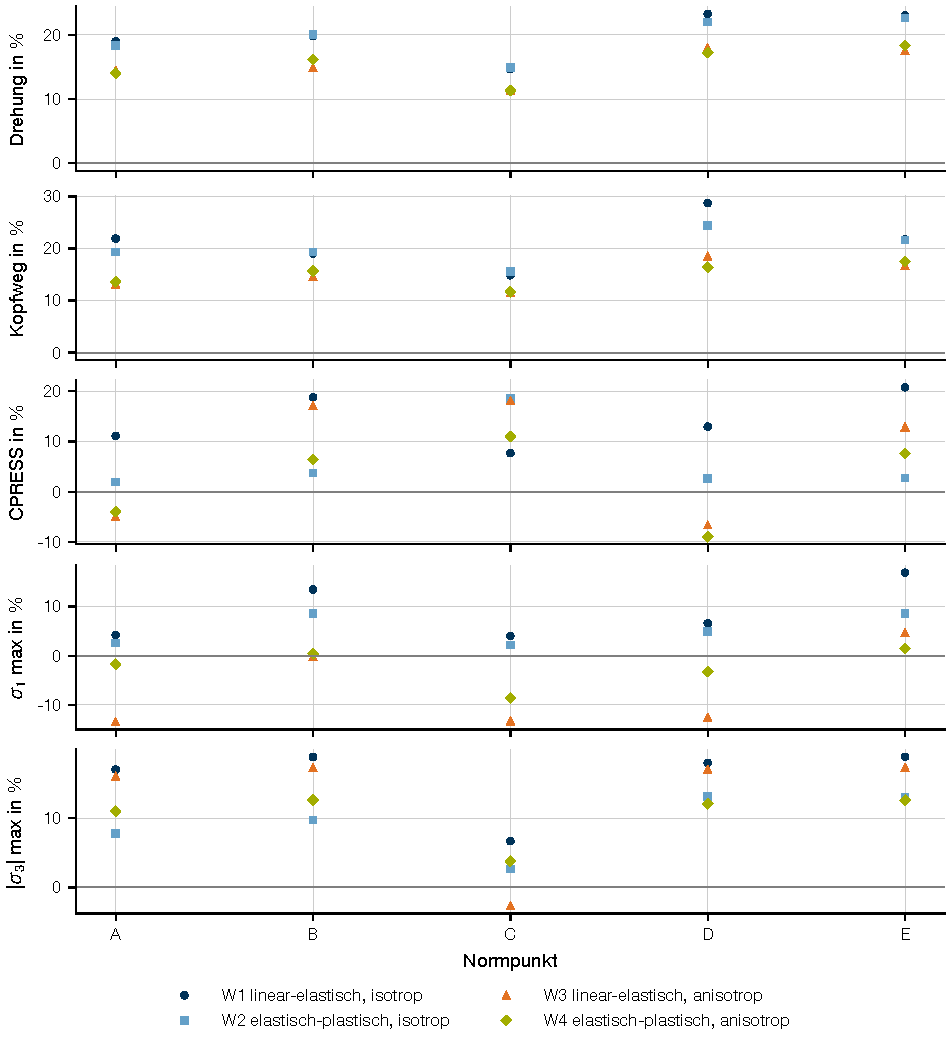
\includegraphics[width=0.8\textwidth]{kap4/koerpereffekt_16nm_qs}
	\caption{Körpereffekt an den Normpunkten A bis E, Taschenkörper gegen Ringkörper gleicher Schichtung, relative Änderung je Werkstoffstufe, $16$\,Nm, quasistatisch. Größtwerte über die Zahnbreite, Marker ohne Linie, weil der Verlauf zwischen den Punkten nicht gerechnet ist.}
	\label{fig:koerpereffekt_16nm_qs}
\end{figure}

% TK erledigt (Gleitobjekt mit !tbp, wird nach der Überarbeitung in der PDF geprüft): Tabelle ist auf mehreren Seiten später dargestellt. Bitte mal überprüfen, woran das liegt, kann sich aber durch die Nachbearbeitungsschleife eh nochmal ändern.

Der Körper verändert die Verformung damit in derselben Größenordnung wie der Wechsel der Werkstoffstufe. Der Taschenkörper nach Zeichnung gilt im Weiteren als Modell des realen Teils, der Ringkörper bleibt die Bezugsgeometrie der Netzstudien aus \secref{sec:netzkonvergenz} und \secref{sec:kopfkante}. Alle weiteren Rechnungen dieser Arbeit, die Fußrundungsvarianten in \secref{sec:fussgeometrie} und die Vollserie für die Bemessung in \secref{sec:stommel_ergebnis}, laufen deshalb auf dem Taschenkörper. Die anisotropen Stufen verwenden dort das CONVERSE-Mapping auf das jeweilige Netz.

% Herkunft:
% Absatz 1 (Einleitung): series_..._qs_gerechnet/analyse/analyse.md Kopf und Abschnitt 1 (99 Stellungen, 395 von 396); fe_simulation_notes.yaml outcome von pilot_..._dy1dy2_AtoE_gerechnet (E 2543 / 3597 MPa; Raten 3 und 60 1/s aus der purpose-Zeile des Piloten); Größtwerte über die Breite: Kopf der Analyse. Stufenbezeichnungen nach Vorgabe; Zitat Sto18 für die Abstufung, Seite in 3.6 prüfen.
% Absatz 2 (Anisotropie linear): series analyse.md Abschnitt 3, Tabelle 16 Nm, Zeilen "Anisotropie (linear)" (Maximum und A bis E).
% Absatz 3 (Plastizität, W4 gegen W2): series analyse.md Abschnitt 3, Tabellen 16 Nm (Plastizität isotrop, Plastizität anisotrop, Anisotropie plastisch) und 8 Nm (sigma1 −31,9 %); Abschnitt 2, Tabelle 16 Nm (86,03 / 52,89 MPa); Fließkurve 4,3 MPa und "nahezu multiplikativ" aus ADR-116 Punkt 47(b).
% Tabelle tab:stufen_16nm: series analyse.md Abschnitt 2 (Größtwerte W1_QS, 16 Nm) und Abschnitt 3 (Spalte Maximum, 16 Nm).
% Absatz 4 (Dehnraten): pilot_..._dy1dy2_AtoE_gerechnet/analyse/analyse.md Abschnitt 8, Tabellen 16 Nm (alle Zahlen), 12 Nm (+40,2 % Kontaktdruck W3 an C, −22,2 % Drehung W4 an C), 8 Nm (Spannen über alle Lastschritte); verlängerter Eingriff aus series analyse.md Abschnitt 4 (0,47 bis 0,60 / 0,35 bis 0,48 Teilungen); Deutung der Lastaufteilung aus dem Tagebuch-outcome des Piloten ("der steifere Werkstoff teilt die Last weniger"), dort auf A bezogen, hier nach den Tabellen auf C.
% Absatz 5 (Definition Schicht- und Körpereffekt): vergleich_koerper_AtoE/analyse.md Einleitung; Schichtmaße aus known_limits.md FE-23 (0,75 gegen 0,667 / 0,786 mm) und fe_simulation_notes.yaml purpose von pilot_..._pocketlevels_..._w1w2 (6 Schichten über |z| ≤ 2,0, 7 je Taschentiefe); 60 Rechnungen je Körper, alle vollständig: outcome von pilot_..._pocket_..._gerechnet und pilot_..._pocketlevels_..._gerechnet, ADR-116 Punkt 48.
% Absatz 6 (Schichteffekt): vergleich_koerper_AtoE/analyse.md "Zusammenfassung der Effekte"; 21 % der Zahnelemente um mehr als 10° aus ADR-116 Punkt 48(a); Folgerung für die Modelldefinition aus known_limits.md FE-23.
% Absatz 7 (Körpereffekt): vergleich_koerper_AtoE/analyse.md "Zusammenfassung der Effekte" (Spannen) und Tabelle 16 Nm, Zeilen W1_QS bis W4_QS (Punktwerte); "der anisotrope Zahn biegt sich weniger, der Steg trägt mehr" aus ADR-116 Punkt 48(b).
% Bild fig:koerpereffekt_16nm_qs: bilder.yaml Eintrag koerpereffekt_16nm_qs; Unterschrift nach vergleich_koerper_AtoE/bildunterschriften.md (koerpereffekt_LOAD_16NM_QS), ohne Doppelpunkt umgestellt.
% Tabelle tab:koerper_spannen: vergleich_koerper_AtoE/analyse.md "Zusammenfassung der Effekte", alle 20 Zeilen.
% Absatz 8 (Folgerung): ADR-116 Punkt 48(b) (Körper wirkt wie der Werkstoffwechsel; Taschenkörper als Modell des realen Teils, Ring als Bezug der Netzstudien) und Punkt 53 (Entscheidung des Nutzers: jede weitere Rechnung auf dem Taschenkörper, Varianten und Vollserie, Mapping je Variantennetz).

\section{Prüfräder vor dem Versuch}
\label{sec:pruefraeder_vorher}

Die Prüfräder wurden vor den Laufversuchen nach dem Verfahren aus \secref{sec:dokumentation_pruefraeder} vermessen. Von den zehn Kernrädern der Laufversuche und den 26 Rädern der Fertigungsstreuung liegen 58 Dateien der Verzahnungsmessung vor, von den sieben Ritzeln der Prüfstandsserie zehn Dateien. In mehreren Runden wurden 21 Räder und drei Ritzel gemessen. Dazu kommen 47 Konturscans von 18 Rädern, je drei Scans des Prüfstandsritzels 95912 und des älteren Ritzels 86481 sowie Rauheitsspuren von 35 Rädern. Sechs Kernräder sind nicht gescannt, für die Ritzel fehlt die Rauheitsmessung.

\tabref{tab:kernraeder_gina} stellt die Kenngrößen der Kernräder denen der Fertigungsstreuung gegenüber. Je Rad zählt die letzte Messung. Die Toleranzen des Messprogramms sind die Werte der Verzahnungsqualität 7 nach DIN 3962 Teil 1 für Teilung, Rundlauf und Profil-Winkelabweichung \cite[S.~3]{DIN3962-1} und nach Teil 2 für die Flankenlinien-Winkelabweichung \cite[S.~1]{DIN3962-2}. Die Dateien nennen die Norm nicht. Sie führen aber deren Größen Teilungssprung und Teilungs-Spannenabweichung über ein Achtel des Umfangs, und die hinterlegten Werte stimmen mit den Tabellen der Norm überein. DIN 3962 ist durch DIN ISO 1328-1 ersetzt, deren Klassen anders gestuft sind \cite[Nationales Vorwort, S.~4 bis 5]{DINISO1328-1}. Die Zeichnung des Rades fordert die Klasse 10 nach DIN ISO 1328-1 (\secref{sec:pruefverzahnung}). Für $d = 52$\,mm, $m_{\mathrm{n}} = 1$\,mm und $b = 15$\,mm ergeben die Gleichungen (5) bis (12) der Norm mit ihren Rundungsregeln die Toleranzen $f_{\mathrm{pT}} = 31$\,µm, $F_{\mathrm{pT}} = 95$\,µm, $f_{\mathrm{H}\alpha\mathrm{T}} = 25$\,µm und $f_{\mathrm{H}\beta\mathrm{T}} = 32$\,µm \cite[S.~36 bis 37]{DINISO1328-1}. Der informative Anhang E nennt die Rundlauftoleranz $F_{\mathrm{rT}} = 85$\,µm \cite[S.~53]{DINISO1328-1}, der informative Anhang G die Toleranz des Teilungssprungs $f_{\mathrm{uT}} = 44$\,µm \cite[S.~60]{DINISO1328-1}. Gezählt werden die Überschreitungen beider Vorgaben.

Die Profil-Winkelabweichung $f_{\mathrm{H}\alpha}$ ist auf beiden Flanken positiv, ihr Mittel je Rad liegt zwischen $5{,}1$ und $18{,}0$\,µm. In jeder der 58 Dateien überschreiten einzelne Zähne die $7$\,µm des Messprogramms. Die Flankenlinien-Winkelabweichung $f_{\mathrm{H}\beta}$ wechselt von Zahn zu Zahn das Vorzeichen und erreicht im Betrag bis zu $107$\,µm. Ihr Mittel über die Zähne bleibt mit $5{,}5$\,µm links und $-4{,}6$\,µm rechts klein. Die Teilungs-Gesamtabweichung $F_{\mathrm{p}}$ überschreitet die $32$\,µm in 40 der 58 Dateien, der Rundlauf $F_{\mathrm{r}}$ die $22$\,µm in 55 Dateien. Das Rad 97345 erreicht mit $F_{\mathrm{p}}$ von $136{,}0$\,µm links und $122{,}9$\,µm rechts, $f_{\mathrm{p}}$ bis $43{,}1$\,µm und $F_{\mathrm{r}}$ von $56{,}9$\,µm die größten Werte der Kerngruppe. Das Rad 97361 folgt mit $80{,}7$ und $79{,}2$\,µm. In der Fertigungsstreuung liegen die vier Räder 97342, 97344, 97348 und 97369 mit $F_{\mathrm{p}}$ über $60$\,µm. Gegen die Klasse 10 der Zeichnung halten neun der zehn Kernräder Teilung und Rundlauf ein, nur das Rad 97345 überschreitet $F_{\mathrm{pT}}$ und $f_{\mathrm{pT}}$. In der Fertigungsstreuung liegen die Räder 97342, 97348 und 97369 über $F_{\mathrm{pT}}$, das Rad 97342 mit $88{,}7$\,µm auch über $F_{\mathrm{rT}}$. Die Profil- und die Flankenlinien-Gesamtabweichung bleiben an allen Rädern unter den $40$ und $48$\,µm der Klasse. Die Flankenlinien-Winkelabweichung einzelner Zähne, auf die Zahnbreite bezogen, überschreitet die $32$\,µm dagegen an acht der zehn Kernräder und an allen 26 Rädern der Fertigungsstreuung. Die Profil-Winkelabweichung einzelner Zähne liegt an einem Kernrad und drei Rädern der Streuung über $25$\,µm. Die Zeichnungsqualität ist damit in Teilung, Rundlauf und Gesamtabweichungen fast durchweg erreicht, in der Flankenlinien-Winkelabweichung einzelner Zähne nicht.

\begin{table}[htbp]
	\caption{Verzahnungsmessung der Räder vor dem Versuch: Mittel, Standardabweichung $s$ und Spanne über die Räder je Gruppe, Flankenwerte links / rechts, je Rad die letzte Messung. Toleranzen der Qualität 7 nach DIN 3962 \cite[S.~3]{DIN3962-1} \cite[S.~1]{DIN3962-2}, wie im Messprogramm hinterlegt (Spalte Q7), und der Klasse 10 nach DIN ISO 1328-1 \cite[S.~36 bis 37, 53 und 60]{DINISO1328-1}, wie die Zeichnung sie fordert (Spalte Q10).}
	\label{tab:kernraeder_gina}
	\centering
	\footnotesize
	\setlength{\tabcolsep}{3pt}
	\begin{tabular}{lllllllll}
		                       &         &          &            & \multicolumn{3}{l}{Kernräder, $n = 10$} & \multicolumn{2}{l}{Fertigungsstreuung, $n = 26$}                                                                         \\
		Größe                  & Einheit & Q7 & Q10  & Mittel                                  & $s$                                              & Spanne                    & Mittel              & $s$                 \\
		\hline
		\arrayrulecolor{black!30}
		$W_{\mathrm{k}}$       & mm      &          &            & $16{,}973$                              & $0{,}006$                                        & $16{,}962$ bis $16{,}984$ & $16{,}982$          & $0{,}004$           \\
		\hline
		$d_{\mathrm{a}}$       & mm      &          &            & $54{,}049$                              & $0{,}015$                                        & $54{,}014$ bis $54{,}068$ & $54{,}070$          & $0{,}013$           \\
		\hline
		$f_{\mathrm{p}}$       & µm      & $10$     & $31$ & $13{,}7$ / $15{,}6$                     & $8{,}9$ / $11{,}5$                               & $7{,}4$ bis $43{,}1$      & $14{,}9$ / $15{,}6$ & $10{,}3$ / $9{,}8$  \\
		\hline
		$f_{\mathrm{u}}$       & µm      & $12$     & $44$ & $15{,}3$ / $16{,}4$                     & $5{,}8$ / $5{,}7$                                & $9{,}5$ bis $31{,}1$      & $17{,}3$ / $18{,}8$ & $7{,}7$ / $10{,}5$  \\
		\hline
		$F_{\mathrm{p}}$       & µm      & $32$     & $95$ & $47{,}9$ / $48{,}0$                     & $36{,}8$ / $31{,}9$                              & $17{,}0$ bis $136{,}0$    & $45{,}6$ / $47{,}4$ & $28{,}4$ / $30{,}2$ \\
		\hline
		$F_{\mathrm{r}}$       & µm      & $22$     & $85$ & $37{,}2$                                & $11{,}6$                                         & $20{,}0$ bis $56{,}9$     & $43{,}3$            & $15{,}7$            \\
		\hline
		$f_{\mathrm{H}\alpha}$ & µm      & $7$      & $25$ & $10{,}3$ / $10{,}2$                     & $2{,}5$ / $1{,}6$                                & $5{,}1$ bis $13{,}3$      & $12{,}9$ / $12{,}7$ & $1{,}8$ / $2{,}2$   \\
		\hline
		$F_{\alpha}$           & µm      &          & $40$ & $18{,}1$ / $17{,}4$                     & $1{,}8$ / $1{,}8$                                & $15{,}4$ bis $21{,}6$     & $17{,}9$ / $17{,}3$ & $1{,}6$ / $1{,}3$   \\
		\hline
		$f_{\mathrm{H}\beta}$  & µm      & $11$     & $32$ & $5{,}5$ / $-4{,}6$                      & $6{,}4$ / $3{,}9$                                & $-12{,}5$ bis $13{,}7$    & $-5{,}1$ / $-1{,}8$ & $8{,}0$ / $8{,}1$   \\
		\hline
		$F_{\beta}$            & µm      &          & $48$ & $21{,}0$ / $20{,}3$                     & $6{,}4$ / $5{,}7$                                & $14{,}1$ bis $34{,}0$     & $21{,}4$ / $24{,}8$ & $5{,}0$ / $6{,}6$   \\
		\hline
		\arrayrulecolor{black}
	\end{tabular}
\end{table}

Die Wiederholmessungen an 21 Rädern grenzen die Messstreuung ab. Zwischen den Runden desselben Rades unterscheiden sich Zahnweite und Kopfkreisdurchmesser im Mittel um $0{,}005$\,mm und $0{,}010$\,mm, die Form- und Profilabweichungen um rund $2$\,µm. Bei $f_{\mathrm{H}\beta}$ links beträgt der mittlere Unterschied $10{,}4$\,µm und bei $F_{\mathrm{p}}$ $9{,}6$\,µm, die größten Spannweiten erreichen $33{,}5$\,µm und $32{,}3$\,µm. Aufbau und Ablauf waren in allen Runden gleich, je Runde wechselte der Bediener. Die Fertigungsstreuung der Steigungs- und Teilungsabweichungen ist deshalb zusammen mit dieser Messstreuung zu lesen. Die Teilungs-Sektorabweichung $F_{\mathrm{pk}}$ nach DIN ISO 1328-1 Anhang D.2 wurde aus den Teilungstabellen nachgerechnet, weil das Messprogramm unter Fpz/8 eine andere Spanne druckt. $F_{\mathrm{pk}}$ liegt auf 43 von 72 Flanken über $22$\,µm, die Programmgröße auf 41. Der Unterschied beider Größen erreicht $22$\,µm.

Die Konturscans der Räder bestätigen die Zahnform der Erzeugung und vermessen die Kopfkante. Der freie Evolventenfit mit dem Nenn-Grundkreis hatte die Profil-Winkelabweichung der Räder als radialen Versatz der Achse von im Median $52$\,µm zum Zahn hin aufgenommen. Dadurch fielen die Radien der Scans rund $50$\,µm zu klein und die Zahndicke rund $28$\,µm zu dünn aus. Mit der an den GINA-Kopfkreis desselben Teils gebundenen Achse beträgt die mittlere quadratische Abweichung (RMS) der Flanken $1{,}8$ bis $3{,}6$\,µm gegenüber $0{,}6$ bis $2{,}1$\,µm des freien Fits. Dieser Wert ist die reale Profilabweichung. Der Fußkreisdurchmesser der Scans weicht je Teil um $-31$ bis $+20$\,µm vom GINA-Wert ab, die Grundkreis-Zahndicke $s_{\mathrm{b}}$ liegt $5$ bis $15$\,µm über dem erzeugten Wert. Die Zahnweite $W_{\mathrm{k}}$ der Kernräder trifft mit $16{,}973$\,mm im Mittel den Wert der STplus-Erzeugung von $17{,}180$\,mm abzüglich $0{,}207$\,mm Zahndickenabmaß. Die Räder der Fertigungsstreuung liegen mit $16{,}982$\,mm $9$\,µm darüber. An der Kopfkante passt ein tangentialer Bogen in 162 von 163 Ecken besser als eine Fase. Sein Radius beträgt im Mittel je Teil $0{,}205$ bis $0{,}248$\,mm. Die Zeichnung des Rades verlangt eine Rundung r $0{,}2$, die STplus-Erzeugung trägt dagegen eine Fase von $45$°.

Die sieben Ritzel der Prüfstandsserie liegen in Teilung und Flankenform eng beieinander. $F_{\mathrm{p}}$ beträgt im Mittel $11{,}8$\,µm links und $10{,}0$\,µm rechts, $F_{\mathrm{r}}$ $13{,}6$\,µm und $f_{\mathrm{p}}$ $1{,}7$\,µm. Über die Toleranzen der Qualität 6 nach DIN 3962, die das Messprogramm hinterlegt, kommen nur wenige Werte. Die Zeichnung von 2022 fordert eine Qualität besser als 6 (\secref{sec:pruefverzahnung}). Der Rundlauf der Ritzel 95911 und 95915 liegt mit $16{,}2$ und $16{,}8$\,µm über $16$\,µm, $f_{\mathrm{H}\beta}$ einzelner Zähne des Ritzels 95920 erreicht $13{,}8$\,µm gegen $8$\,µm. Dazu kommt $f_{\mathrm{H}\alpha}$ der ersten Messrunde mit $5{,}2$ bis $7{,}0$\,µm, das in der zweiten Runde mit $-1{,}1$ bis $1{,}7$\,µm gemessen wurde. Die Kopfrücknahme liest das Messprogramm je Zahn mit $-22{,}2$ bis $-25{,}8$\,µm zwischen den Durchmessern $51{,}946$ und $52{,}880$\,mm, im Mittel $-23{,}3$\,µm links und $-23{,}7$\,µm rechts. Die Zahnweite streut mit einer Standardabweichung von $0{,}048$\,mm um $16{,}808$\,mm und liegt $4$\,µm unter dem erzeugten Wert von $16{,}812$\,mm. Zwischen den Runden schwankt sie beim Ritzel 95918 um $0{,}127$\,mm, Teilung und Rundlauf wiederholen innerhalb von $4{,}5$\,µm. Die Zeichnung von 2022 schreibt die Kopfrücknahme mit $25$\,µm linear ab dem Durchmesser $51{,}946$\,mm und die Zahnweite $16{,}822$\,mm mit dem Abmaß $-0{,}021$\,mm vor (\secref{sec:pruefverzahnung}).

Der Konturscan des Prüfstandsritzels 95912 ist die Gegenprobe des Achsverfahrens am Stahl. Die Bindung an den GINA-Kopfkreis verschiebt die Achse hier um $4$ bis $15$\,µm gegen $30$ bis $69$\,µm bei den gespritzten Rädern. Der Fußkreis stimmt mit $48{,}308$\,mm gegen $48{,}299$\,mm auf $9$\,µm. Die Zahndicke liegt $23$\,µm unter dem erzeugten Wert, wie es die Zahnweite $16{,}786$\,mm dieses Ritzels erwarten lässt. Die Rücknahme am Kopf liest der Scan mit $25{,}3$ bis $27{,}1$\,µm gegen $-22{,}7$ und $-23{,}4$\,µm der GINA-Messung. Die Kopfkante des Ritzels ist in \secref{sec:kopfkante} beschrieben. Das ältere Ritzel 86481 trägt eine Rücknahme von $20{,}8$\,µm und dient wegen seines um $0{,}17$\,mm tieferen Fußkreises nicht als Bezug (\secref{sec:pruefverzahnung}).

% TK erledigt (Kante nur noch in 4.2, 86481 nur noch in 3.1 beschrieben): Der Inhalt des Abschnitts ist schon mehr oder weniger an anderer Stelle genauso beschrieben. Bitte nur an einer Stelle das Ritzel in dem Ausmaß beschreiben. 

Die Rauheit der Zahnflanken wurde mit drei Spuren je Flanke gemessen, der Wert einer Flanke ist das Mittel der Spuren. Die Kernräder haben $R_{\mathrm{a}}$ von $0{,}81$\,µm links und $0{,}93$\,µm rechts bei Standardabweichungen von $0{,}32$ und $0{,}44$\,µm sowie $R_{\mathrm{z}}$ von $4{,}9$ und $5{,}8$\,µm. Die Räder der Fertigungsstreuung liegen mit $R_{\mathrm{a}}$ von $1{,}20$\,µm und $R_{\mathrm{z}}$ von $7{,}3$\,µm auf beiden Flanken darüber. Innerhalb der Fertigungsstreuung trennen sich zwei Gruppen nach Messtag und Bediener. Die am 12. und 21. Mai gemessenen Räder 97341 bis 97356 dieser Gruppe sowie 97371 liegen bei $R_{\mathrm{a}}$ von $1{,}2$ bis $1{,}9$\,µm. Die am 27. Mai unter dem Chargenlabel der Prüfverzahnung kst-E gemessenen Räder 97357 bis 97374 liegen bei $0{,}4$ bis $1{,}6$\,µm. Beide Gruppen stammen aus derselben Charge und demselben Messverfahren und wurden von zwei Bedienern aufgenommen. Ein anderer Unterschied besteht nicht. Je ein Protokoll der Verzahnungs- und der Rauheitsmessung steht als Beispiel in \anhref{sec:anhang_g}.

Für das FE-Modell mit gemessener Geometrie werden die Zahndicken aus den GINA-Zahnweiten übernommen, nicht aus den Scans. Die Grundlinie behält die in STplus erzeugte Zahndicke. Die Kopfrundung des Rades von $0{,}21$\,mm und die Kopfrücknahme des Ritzels gehen als örtliche Anpassungen ein, die Kopfkante des Ritzels bleibt nach \secref{sec:kopfkante} ein Parameter des Modells. Die Scans der gelaufenen Räder werden in \secref{sec:schadensbilder} mit dem Band aller Scans vor dem Versuch verglichen. Der Vergleich desselben Zahns setzt dieselbe Messebene voraus, deren Lage zur Stirnfläche des $15$\,mm breiten Zahns in den Dateien nicht festgehalten ist (beim Rad 97340 stimmt sie mit $85{,}95$\,mm überein). Die 30 Scans vom 23. Juni mit rund 400 Punkten bleiben aus der Kantenstatistik ausgeschlossen.

% TK erledigt (Absatz neu sortiert: Zahndicke, Kopfrundung und Rücknahme, Nachher-Scans, Kantenstatistik; Schliffbild und CT nur im Ausblick): Der letzte Abschnitt ist etwsa wirr formuliert und nimmt viele unterschiedliche Themen auf. Bitte klarer sortieren und aktualisieren auf den jetzigen Stand. Wenn da Fragen sind, bitte fragen.

% Herkunft:
% Absatz 1 (Umfang): architecture_decisions.md ADR-117 Consequences (10 Kernräder, 26 Räder der
%   Fertigungsstreuung, 7 Ritzel, 86481; Lücken) und Amendment 2026-10-12 Punkt 4 (Scan 95912);
%   80_output/messungen/gina/wheel/toleranzen_protokoll.md (58 Dateien) und gina/pinion/toleranzen_protokoll.md
%   (10 Dateien); gina/wheel/wiederholbarkeit.md (21 Teile), gina/pinion/wiederholbarkeit.md (3 Teile);
%   konturscan/wheel/bericht.md Tabelle "Je Scan" (47 Zeilen, 18 Teile) und konturscan/pinion/bericht.md
%   (je drei Scans 95912 und 86481); rauheit/wheel/gruppen.md (n 10 + 25); known_limits.md MEAS-04.
% Absatz 2 und Tabelle tab:kernraeder_gina: gina/wheel/tabelle_streuung.md (Mittel, s, min, max je Gruppe);
%   gina/wheel/toleranzen_protokoll.md Tabelle 1 (Toleranzen, Stufe) und Abschnitt "Überschreitungen"
%   (Werte und Dateien je Label; Einzelzeilen für 97345, 97361 -neu1, 97342, 97344, 97348, 97369 und
%   97344 rechts Zahn 1 = -107,2); known_limits.md MEAS-05 (2026-10-25 geschlossen: die Werte des Messprogramms
%   sind die Tabellen der DIN 3962 Teil 1 S. 2 und 3 und Teil 2 S. 1, an der Norm geprüft); Klasse 10 nach
%   DIN ISO 1328-1 aus gearcore.measurement.tolerances (Gl. (5) bis (12) S. 36 bis 37, Anhang E.1 S. 53, Anhang G.2
%   S. 60), Überschreitungen aus gina/wheel/toleranzen_protokoll.md Abschnitt Zeichnungsqualität (Kernräder: fp/Fp/fHa
%   nur 97345, fHb 8 von 10; Streuung: Fp 97342/97348/97369, Fr 97342 88,7, fHa 97342/97348/97364, fHb 26 von 26);
%   F_alphaT 40 und F_betaT 48 der Klasse 10 gegen die Spannen 15,4 bis 21,6 und 14,1 bis 34,0 der Tabelle.
% Absatz 3: gina/wheel/wiederholbarkeit.md ("Spannweite je Größe"); ADR-117 Amendment
%   2026-10-10 Punkt 4 und known_limits.md MEAS-08 (gleicher Aufbau, Bedienerwechsel);
%   gina/wheel/teilungssektoren.md (Kopf, Schlusszeile 41/43 von 72, 97348 rechts 78,1 gegen 100,1);
%   gina/wheel/fenster_zaehne.md (Spalte Rang: 97363 links, 97368 links Rang 1; Kernräder).
% Absatz 4: konturscan/wheel/bericht.md Kopf (Achsbindung, 52 µm, 50 µm, 28 µm), "Je Scan" (RMS Flanken
%   1,8 bis 3,6, frei 0,6 bis 2,1), "Je Teil" (d_f gegen GINA, s_b − erzeugt 5 bis 15, ρ Mittel 0,205 bis
%   0,248); gina/wheel/tabelle_streuung.md (W_k je Gruppe); ADR-117 Amendment
%   2026-10-12 Punkt 1 (17,180 − 0,207, +9 µm) und 2026-10-11 Punkt 2 (Zeichnung r 0,2, STplus 45°);
%   known_limits.md MEAS-11 (162 von 163 Ecken).
% Absatz 5: gina/pinion/tabelle_streuung.md (Mittel, s, W_k); gina/pinion/toleranzen_protokoll.md
%   (Toleranzen Stufe 6, Überschreitungen Fr, fHb 95920, fHa erste Runde); gina/pinion/wiederholbarkeit.md
%   (fHa zweite Runde, WK 95918 0,127, Fp/Fr max 4,4/4,5); gina/pinion/kopfruecknahme_ritzel.md (fKo je Zahn,
%   Beginn/Ende); ADR-117 Amendment 2026-10-12 Punkt 3 (16,808 gegen 16,812).
% Absatz 6: konturscan/pinion/bericht.md ("Je Scan" Versatz 15/4/5, ρ 0,004/0,006, Gerade 25,3 bis 27,1;
%   "Je Teil" d_f, s_b − erzeugt, 86481); ADR-117 Amendment 2026-10-12 Punkt 4 (Zahnweite 16,786,
%   Mikroskopbilder, 86481 anderer Schnitt, nicht Bezug von V2); known_limits.md MEAS-06.
% Absatz 7: rauheit/wheel/gruppen.md (Mittel, s, min, max); rauheit/wheel/tabelle.md
%   (Messtage und Chargenlabel je Rad); known_limits.md MEAS-04 (Ritzel ohne
%   Rauheit); ADR-117 Amendment 2026-10-11 Punkt 5 (Protokolle im Anhang).
% Absatz 8: ADR-117 Amendment 2026-10-12 Punkt 3 (Zahndicke aus Zahnweiten, V0/V1 STplus, Rundung und
%   Rücknahme örtlich); known_limits.md MEAS-06 (Kante bleibt Modellparameter), MEAS-10 (Messebene),
%   MEAS-03 (30 Scans vom 23.06.: 97363, 97364, 97367 bis 97374).
% Bildwunsch: 80_output/messungen/gina/wheel/zaehne_97345-neu.svg, Teilung und Rundlauf je Zahn des Kernrades
%   97345 mit dem Fenster der Zähne 36 bis 40 (größtes F_p der Kerngruppe); als Gegenstück zaehne_97366-neu.svg
%   (kleinstes F_p).
% Bildwunsch: GINA-Streuung der Räder (F_p, F_r, f_Halpha, W_k je Rad, Kerngruppe gegen Fertigungsstreuung),
%   noch zu zeichnen aus gina/wheel/tabelle_streuung.csv und den .mew-Werten (M6).
% Bildwunsch: Teilungssektoren Fpz/8 des Messprogramms gegen F_pk je Flanke aus gina/wheel/teilungssektoren.md,
%   noch zu zeichnen (M6).
% Bildwunsch: 80_output/messungen/konturscan/wheel/kopfkante_97340_97340-Z1.svg, Kopfrundung des Rades
%   (Messpunkte, scharfe Ecke, Bogen- und Fasenfit, Kernrad 97340, Zahn 1).
% Bildwunsch: 80_output/messungen/konturscan/wheel/ueberlagerung_97340_97340-Z1.svg, Zahnform des Rades gegen
%   die Erzeugung mit überhöhter Abweichung.
% Bildwunsch: 80_output/messungen/konturscan/pinion/ueberlagerung_pinion_rig_series.svg und
%   ueberlagerung_pinion_older.svg, Ritzel 95912 und 86481 gegen die Erzeugung (Kopfrücknahme, Fußkreis).
% Bildwunsch: Rauheitsgruppen R_a und R_z je Rad nach Gruppe, Messtag und Chargenlabel aus
%   rauheit/wheel/tabelle.md, noch zu zeichnen (ADR-117: bisher kein Rauheitsbild vorgesehen, Protokolle im
%   Anhang; Nutzer entscheidet).

\section{Temperaturverhalten am Prüfstand}
\label{sec:temperatur}

Vor den Laufversuchen wurde am Rad 97351 die auf der Zahnflanke gemessene Zahnmassentemperatur über dem Drehmoment und der Drehzahl nach \secref{sec:auswertung_laufversuche} aufgenommen. Ziel war die Einstellung der Öltemperatur für die Zahnmassentemperatur von $80$\,\textdegree C. Die Öltemperatur an der Messstelle vor der Prüfverzahnung betrug $75$\,\textdegree C. \figref{fig:temperatur_matrix_97351} zeigt die sechs Werte als Balken gegen den Bezug von $80$\,\textdegree C.

% TK erledigt (nur noch ME-Nummern): Die Bezeichnungen der Excel mit kst-E_ bitte überall rausnehmen und immer nur mit der ME Nummer arbeiten.

\begin{figure}[htbp]
    \centering
    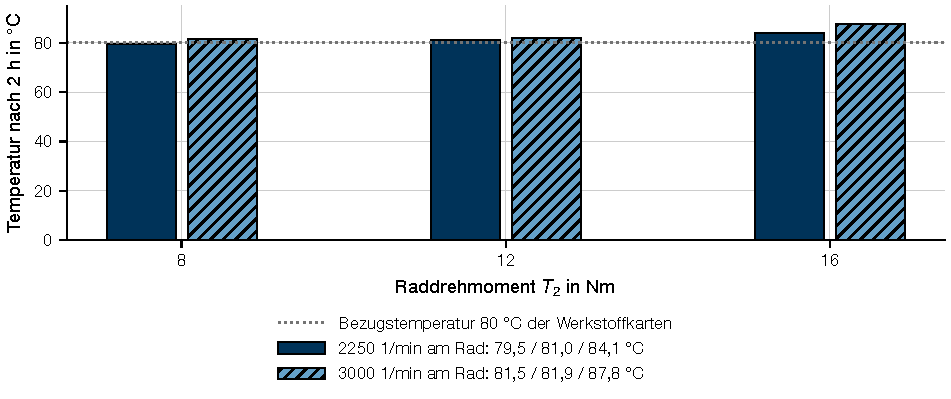
\includegraphics[width=\textwidth]{kap4/temperatur_matrix_97351}
    \caption{Zahnflankentemperatur nach zwei Stunden am Rad 97351 über dem Raddrehmoment bei $2250$ und $3000$\,1/min am Rad, Öltemperatur $75$\,\textdegree C an der Messstelle, Wärmebildkamera mit Emissionsgrad $1$, Bezug $80$\,\textdegree C.}
    \label{fig:temperatur_matrix_97351}
\end{figure}

% TK (folgt mit Paket B3, Bild wird neu gezeichnet): Den Balken fehlt ein Muster für schwarz weiß und auch hier weider das Grid in den Hintergrund bringen. Balken gerne auch etwas dünner. Sieht so platzeinnehmend aus, obwohl die Grafik am Ende wenig aussagt, also nicht minimalprinzip meiner Meinung nach.

\figref{fig:waermebild_16nm_3000} zeigt als Beispiel die Aufnahme bei $16$\,Nm und $3000$\,1/min mit dem Messpunkt auf der Zahnflanke. Die übrigen fünf Aufnahmen stehen in \secref{sec:anhang_h}.

\begin{figure}[htbp]
    \centering
    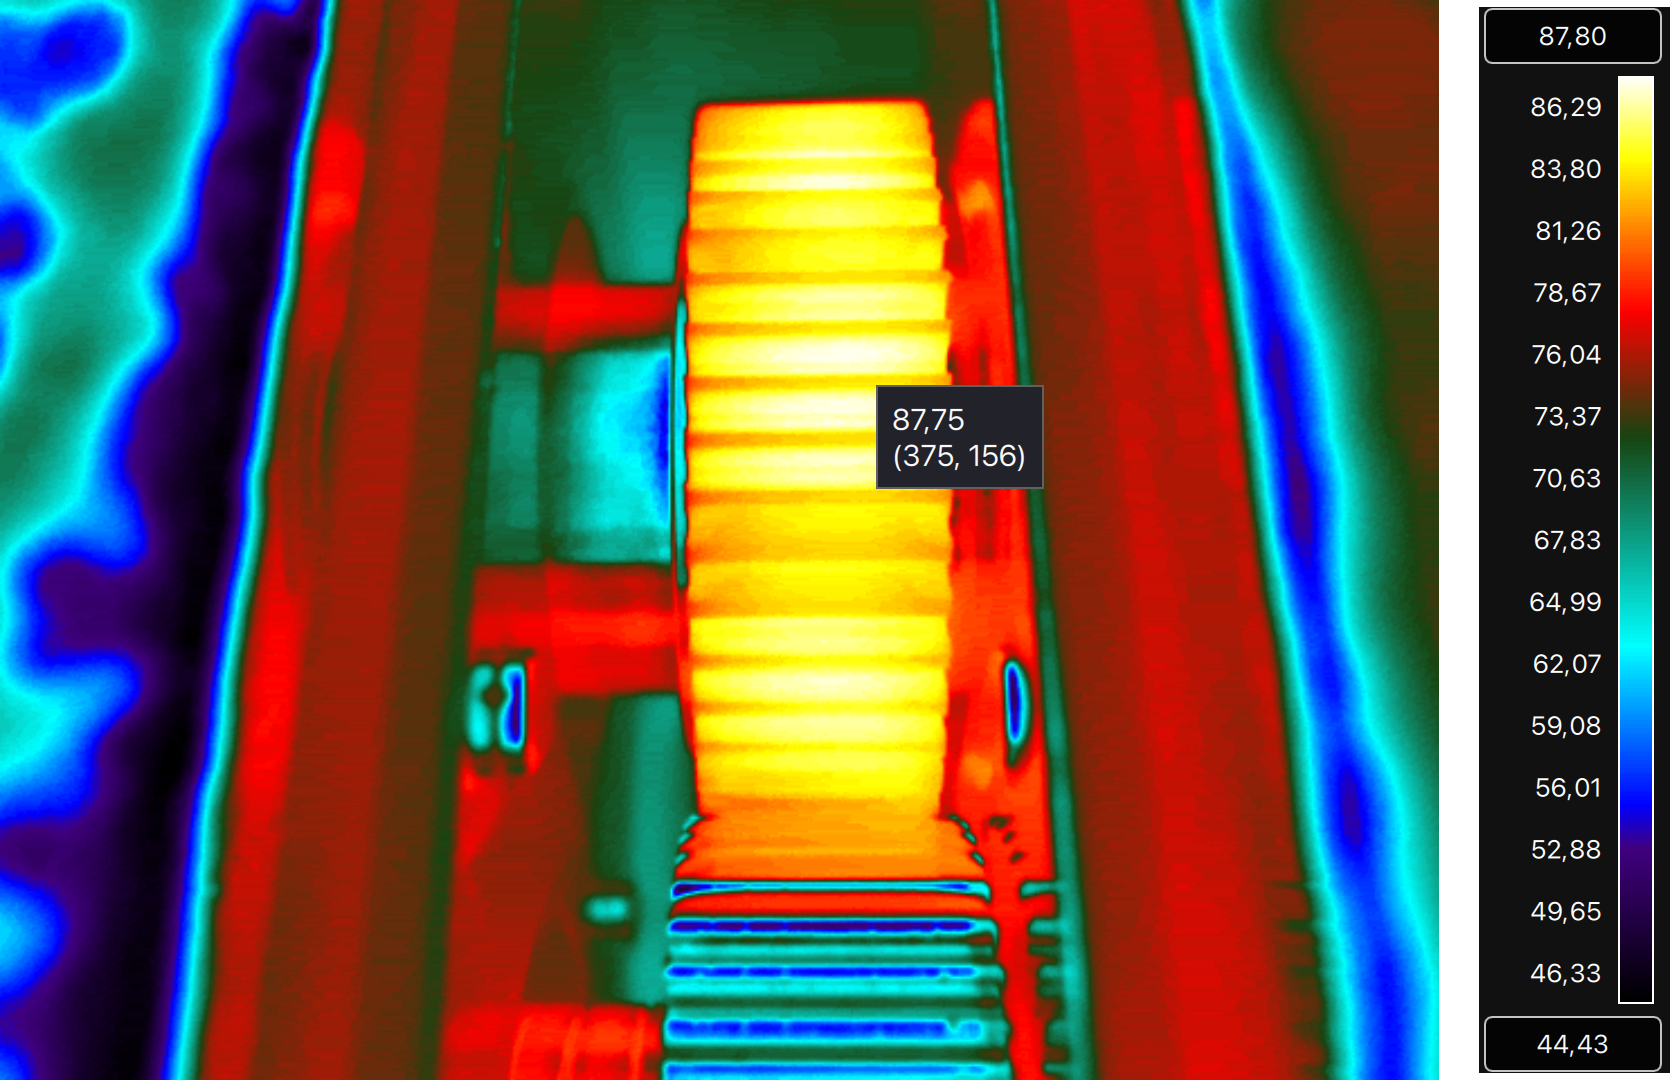
\includegraphics[width=0.8\textwidth]{kap4/waermebild_16nm_3000}
    \caption{Wärmebildaufnahme des Rades 97351 nach zwei Stunden bei $16$\,Nm und $3000$\,1/min am Rad, Emissionsgrad $1$. Der Messpunkt liegt auf der Zahnflanke, die Legende nennt die Temperaturspanne der Aufnahme.}
    \label{fig:waermebild_16nm_3000}
\end{figure}

Bei $8$ und $12$\,Nm liegt die Flankentemperatur mit $79{,}5$ bis $81{,}9$\,\textdegree C innerhalb von $2$\,K um den Bezug. Bei $16$\,Nm steigt sie auf $84{,}1$\,\textdegree C bei $2250$\,1/min und auf $87{,}8$\,\textdegree C bei $3000$\,1/min. Die höhere Drehzahl trägt zwischen $0{,}9$\,K bei $12$\,Nm und $3{,}7$\,K bei $16$\,Nm bei. Der Schritt von $8$ auf $16$\,Nm bringt bei $3000$\,1/min $6{,}3$\,K. Die Öltemperatur von $75$\,\textdegree C hält den Bezug damit auf den Stufen $8$ und $12$\,Nm, auf der Stufe $16$\,Nm läuft der Zahn wärmer. In den Läufen bei $16$\,Nm wurde die Solltemperatur an der Messstelle deshalb auf $67$\,\textdegree C gesetzt (vgl. \tabref{tab:versuchsprogramm_pa46}). Maßgebend ist die Zahnmassentemperatur von $80$\,\textdegree C, auf die alle Versuche an dieser Verzahnung bezogen sind, auch die anderer Lehrstühle. Eine Kastentemperatur wurde in der Matrix nicht aufgezeichnet. Nach der Matrix lief das Rad bei $12$\,Nm weiter und versagte nach $2{,}42 \cdot 10^{6}$ Lastwechseln über alle Stufen mit den vollständig abgebrochenen Zähnen 34 bis 41 (\secref{sec:schadensbilder}). Dieser Lauf trägt eine gestufte Vorgeschichte und erscheint in \secref{sec:woehlerlinien} nur als Marker.

% Herkunft:
% Absatz 1 und 2 (Matrix): 70_input/72_Kleingetriebepruefstand_KV3/kst-E_Laufversuche_KV3.xlsx, Zeilen 77 bis 83
%   (kst-E_63, Rad 97351, Ritzel 95919, Öltemperatur 75, Ziel 80, Ritzelmoment 11,8/7,9/7,8/15,7 Nm, Drehzahl
%   2294 und 3058 1/min am Ritzel = 2250 und 3000 am Rad, Bemerkung "nach 2h ... °C Zahnflankentemperatur mit
%   Emissionsgrad 1"); 80_output/messungen/woehler/vergleich.md Tabelle "Temperaturmatrix kst-E_63" (2250:
%   79,5/81,0/84,1; 3000: 81,5/81,9/87,8 °C); Bild temperatur_matrix_97351 (measurements.py woehler, L4).
%   Wärmebildkamera, Öltemperatur = Messstelle vor der Prüfverzahnung, Weiterlauf bei 12 Nm bis zum Ende:
%   Nutzer 2026-10-18 (ADR-118 Amendment vom Abend, Punkt 4 und 5). Differenzen: Drehzahl 2,0/0,9/3,7 K,
%   Drehmoment bei 3000 1/min 6,3 K. 67 °C der Läufe 70 bis 73: Spalte G der Mappe. Endzahl 2 424 628:
%   Spalte S Zeile 83; "5-6 kaputte Zähne": Spalte T Zeile 83. VDI 2736 Blatt 4 Abschnitt 8.2: über 3.8.
%   67 °C und Emissionsgrad: Nutzer 2026-10-18 (Vorversuche zeigten bei erhöhtem Moment deutlich höhere
%   Zahnmassentemperaturen; Vereinbarung mit anderen Lehrstühlen auf 80 °C; Emissionsgrad 1 aus einem Vorversuch
%   der Forschungsstelle mit Messstreifen); Wärmebilder: 70_input/72_Kleingetriebepruefstand_KV3/Bilder/
%   Waermebildaufnahme_Kunststoffraeder/<T>_<n>.png, geschnitten mit scripts/thesis_thermal_images.py.
% Bildwunsch: kap4/temperatur_matrix_97351, kap4/waermebild_16nm_3000 (bilder.yaml); die übrigen fünf in Anhang H.
% Bibwunsch: keiner.
% Nomenklatur: keine neuen Zeichen.
% Offen: Kastentemperatur der Matrix (nicht aufgezeichnet).
